
\chapter{Ergebnisse und Diskussion}
     Im Rahmen dieser Studienarbeit wurden verschiedene Parameterstudien zur Modellierung der nichtkatalytischen Partialoxidation (POx) von Erdgas durchgeführt und hinsichtlich verschiedener Eigenschaften miteinander zu verglichen. 
     \section{Wahl des Reaktionsmechanismus}
        \label{sec:auswertung_mechanismus}
        Wie in Kapitel \ref{sec:reaktionsmechanismen_literatur} beschrieben, wurden die in dieser Studienarbeit eingesetzten Reaktionsmechanismen nicht speziell für die partielle Oxidation, sondern für Verbrennungsprozesse von Kohlenwasserstoffen entwickelt. Deshalb besteht die Notwendigkeit einer Validierung und eines Vergleichs der eingesetzten Mechanismen.
        Da alle Simulationen der verschiedenen Reaktionsmechanismen in einem identischen Reaktornetzwerk unter konstanten Bedingungen durchgeführt wurden, ist ein Vergleich der Gaszusammensetzungen am Reaktorausgang möglich. In Abbildung \ref{fig:auswertung_vergleich_exp_stoffe} sind diese Zusammensetzungen für beide simulierten Fälle dargestellt. Zur verbesserten Darstellung wurde der Maßstab des Methans um das Zehnfache vergrößert.
        \begin{figure}[H]
            \centering
            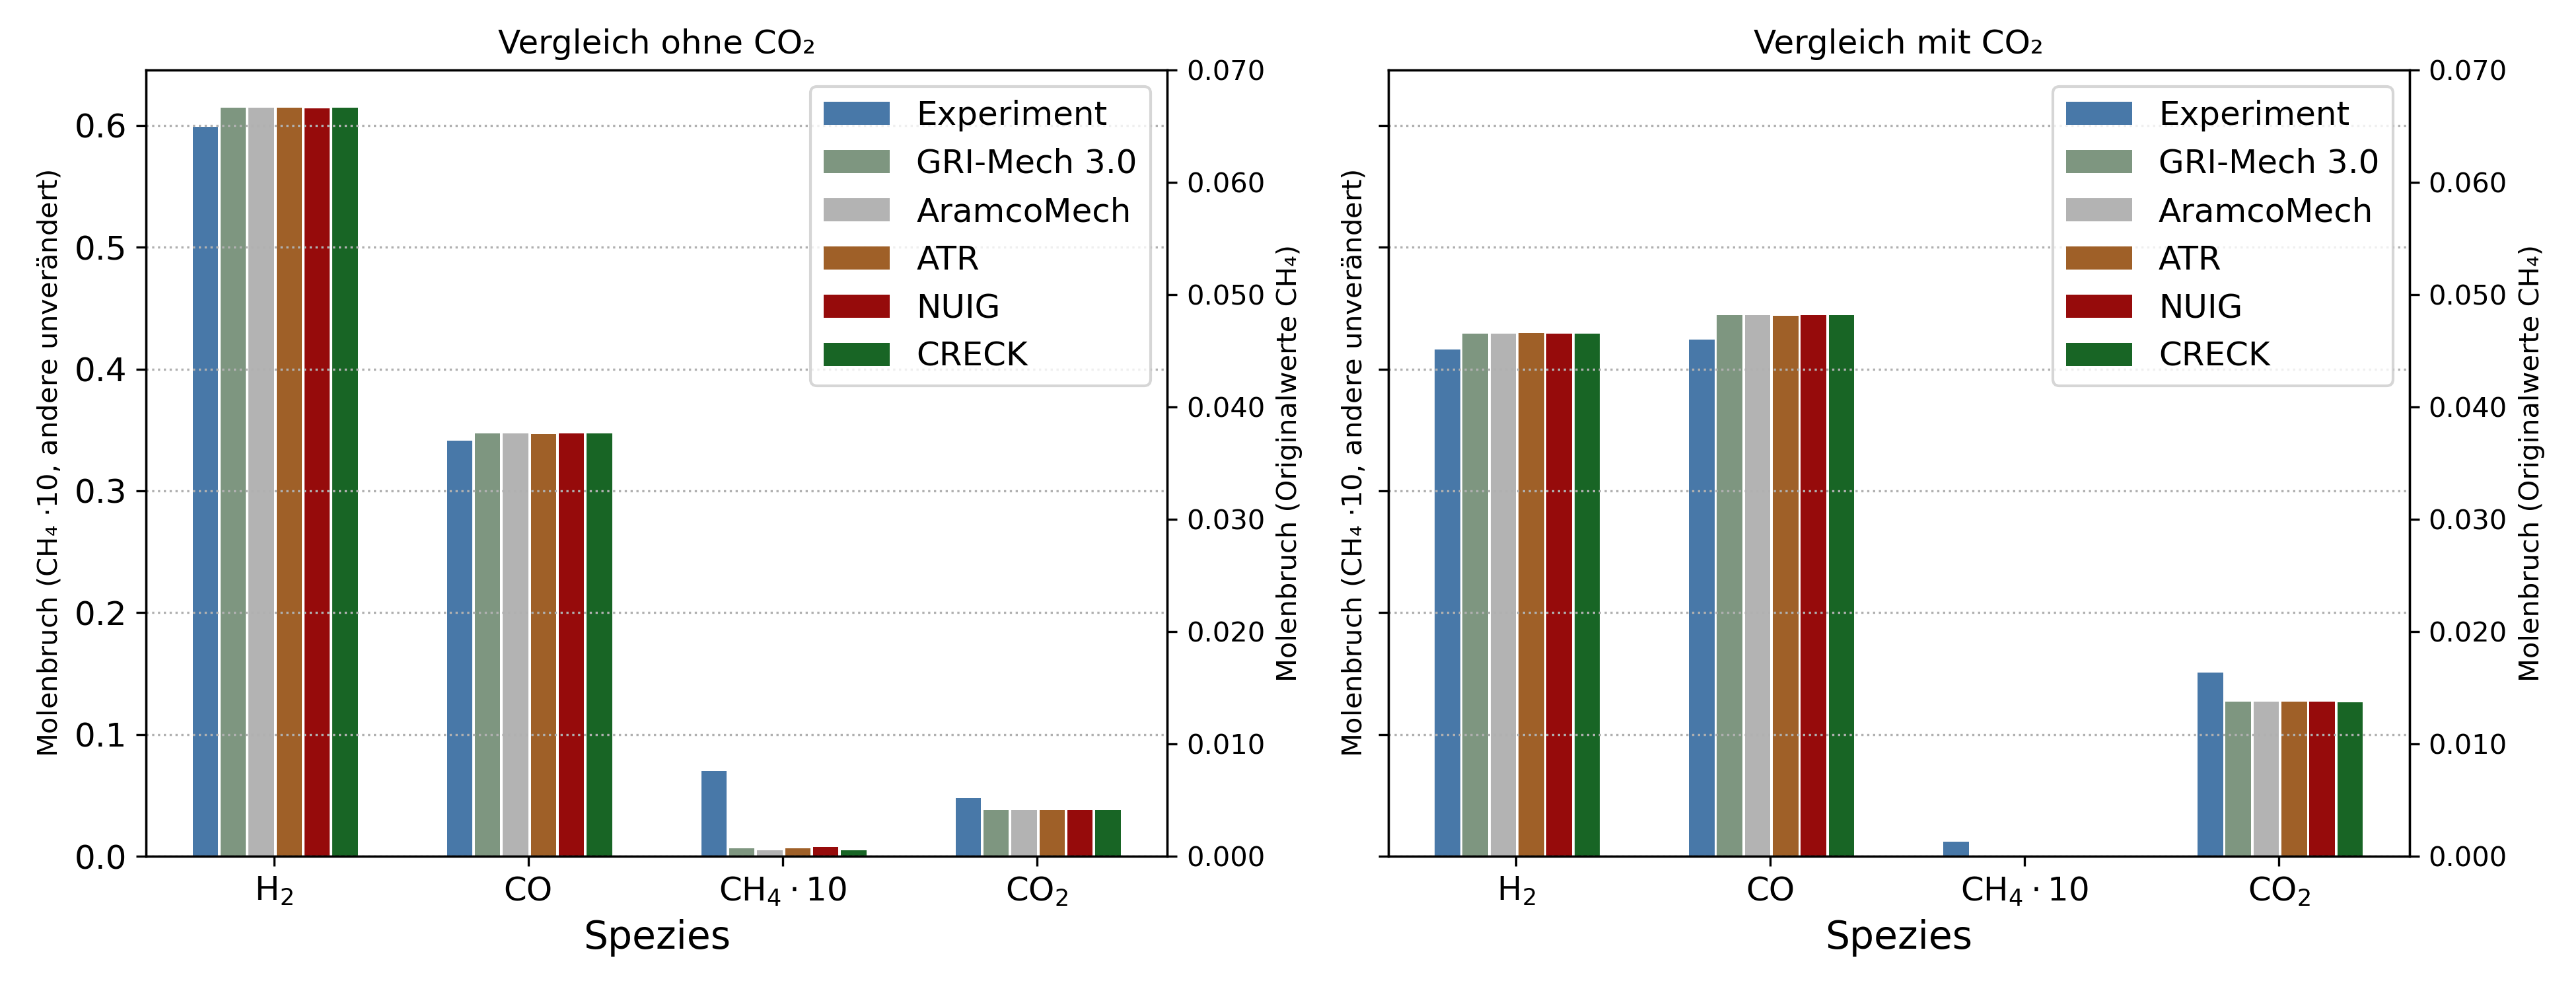
\includegraphics[width=1\linewidth]{img/Vergleich_mech/vergleich_Experimentaldaten_scaled_CH4_gap.png}
            \caption{Vergleich der Massenanteile der Spezies CO, CO$_2$, H$_2$ und CH$_4$ im Produktgas anhand der Berechnungen verschiedener $\mbox{Reaktionsmechanismen}$}
            \label{fig:auswertung_vergleich_exp_stoffe}
        \end{figure}
        Mit der mittleren quadratischen Abweichung (mean squared error, MSE) kann abgeschätzt werden, wie weit ein Wert um einen wahren Wert streut. Dieser ist durch 
        \begin{align}
            MSE = \frac{1}{n}\sum^n_{i=1}\left( Y_i - \hat{Y}_i\right)^2
            \label{eq:mse}
        \end{align}
        definiert, wobei $n$ die Anzahl der Datenpunkte, $Y_i$ die simulierten Werte und $\hat{Y}_i$ die Experimentalwerte sind. 
        In Tabelle \ref{tab:auswertung_mse_mechanismen} sind die mittleren quadratischen Abweichungen beider Simulationen zusammengefasst dargestellt.
        \begin{table}[H]
            \centering
            \caption{Gesamtfehler (mittlerer quadratischer Fehler, MSE) der betrachteten Reaktionsmechanismen für beide Betriebsweisen}
            \label{tab:auswertung_mse_mechanismen}
            \begin{tabular}{lcc}
                \toprule
                \textbf{Mechanismus} & \textbf{Gesamt-MSE (kein CO$_2$)} & \textbf{Gesamt-MSE (mit CO$_2$)} \\
                \midrule
                GRI-Mech 3.0   & 0{,}00006 & 0{,}00023 \\
                AramcoMech         & 0{,}00004 & 0{,}00026 \\
                ATR-Mechanismus & 0{,}00006 & 0{,}00023 \\
                NUIG           & 0{,}00004 & 0{,}00022 \\
                CRECK          & 0{,}00003 & 0{,}00029 \\
                \bottomrule
            \end{tabular}
        \end{table}
        Es ist erkennbar, dass es nur sehr geringe Abweichungen zwischen den Ergebnissen der Mechanismen gibt. In der Literatur sind oftmals Unterschiede zwischen verschiedenen Reaktionsmechanismen beschrieben, allerdings beziehen sich diese Unterschiede oftmals auf direkte Flammeigenschaften wie die Zündverzögerung. Durch die Nachbrennzone gibt es allerdings eine Annäherung der Stoffe an ein chemisches Gleichgewicht. Da diese Gleichgewichtsreaktionen langsamer ablaufen, unterliegt die Parametrisierung dieser Gleichgewichte weniger Ungenauigkeiten, weshalb sich sehr ähnliche Ergebnisse ergeben. 

        Um die Abweichungen der Mechanismen festzustellen, ist eine gesonderte Betrachtung erforderlich. In Abbildung \ref{fig:temp_ch4} sind die Temperatur sowie der Methangehalt am Anfang des PFRs dargestellt. 
        \begin{figure}[H]
            \centering
            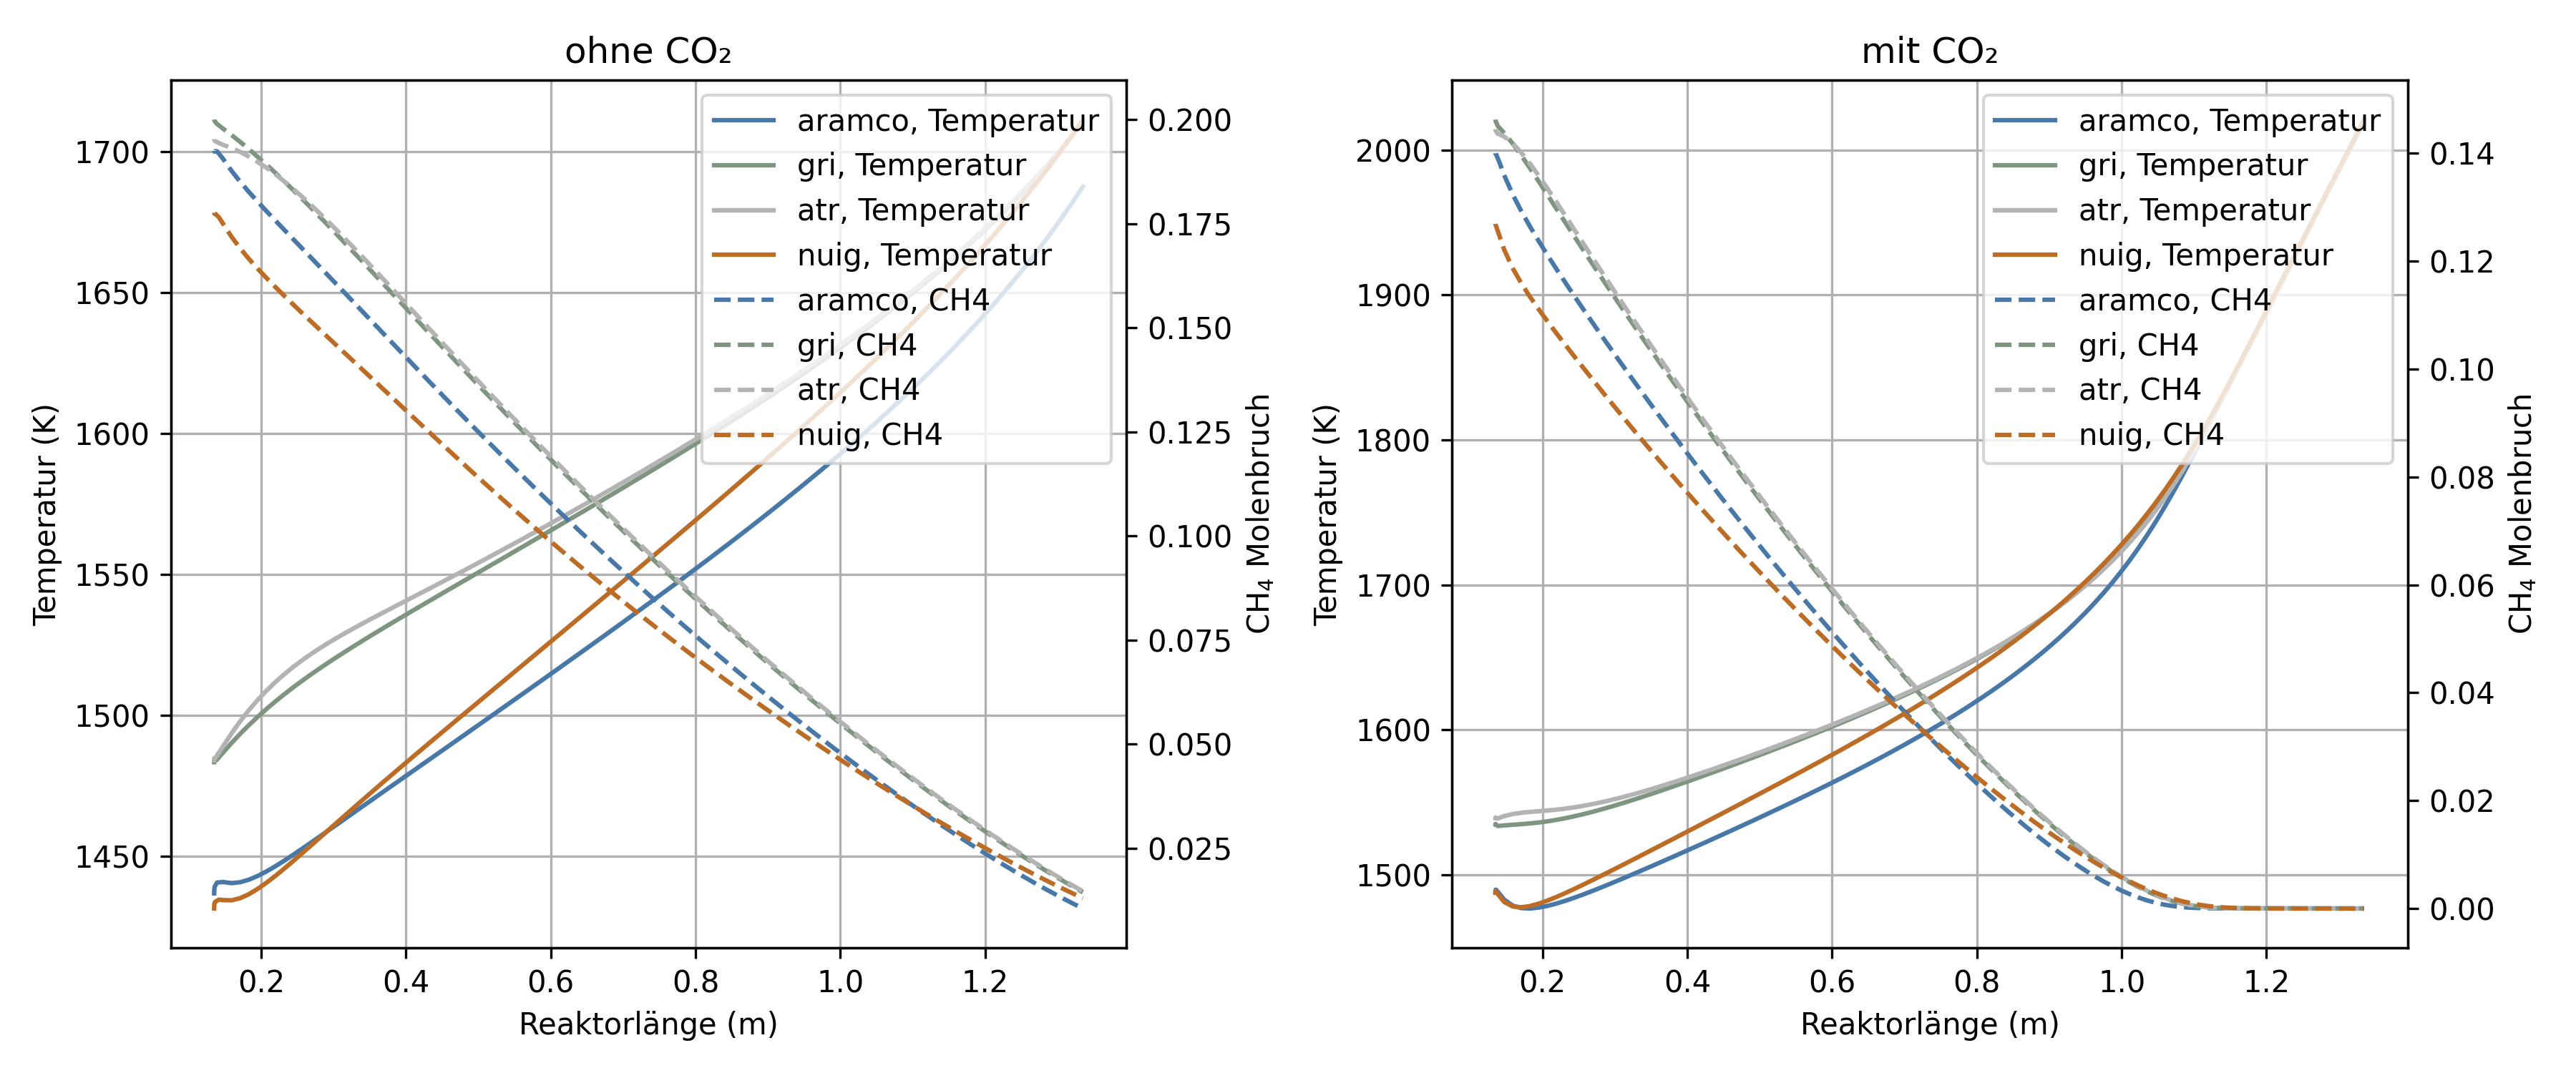
\includegraphics[width=1\linewidth]{img/Vergleich_mech/Temp_CH4.png}
            \caption{Temperatur und Methangehalt im Reaktor zur Unterscheidung der Flammeigenschaften verschiedener Mechanismen}
            \label{fig:temp_ch4}
        \end{figure}
        Dabei ist eine klare Abweichung der Mechanismen untereinander zu erkennen. Da jedoch keine Daten aus Versuchen vorliegen, ist eine Einschätzung der Güte nicht möglich. Dabei ist auch erkennbar, dass durch den höheren Volumenstrom im Fall der CO$_2$-Zugabe eine deutlich kürzere Flammzone vorliegt. Somit stellen sich die Gleichgewichte im zweiten Fall deutlich schneller ein. 

        Auffällig in Tabelle \ref{tab:auswertung_mse_mechanismen} ist, dass die Ergebnisse der Simulationen mit CO$_2$-Zugabe einer höheren Ungenauigkeit unterliegen als die Ergebnisse der Referenzvariante. Zum einen ist dies dadurch erklärbar, dass die verwendeten Reaktionsmechanismen ursprünglich für Anwendungen in der Verbrennung entwickelt wurden. Die CO$_2$-haltigen Gleichgewichte (u. a. die Wassergas-Shift-Reaktion) sind daher nicht optimal parametrisiert, da sie bei der Validierung unter stöchiometrischen Flammenbedingungen nur eine geringe Rolle spielen. Zum anderen führt die Zugabe von CO$_2$ zu einem höheren Massen- und Volumenstrom, wodurch sich die Verweilzeit im Reaktor verkürzt. Dadurch können sich Gleichgewichtsreaktionen nicht vollständig einstellen, was eine größere Abweichung verursacht.
        
        Um einen erheblichen Unterschied der Reaktionsmechanismen festzustellen, wäre ein direkter Vergleich der Flammzone notwendig. Hinsichtlich der großen Ähnlichkeit der Ergebnisse ist eine Erklärung der Abweichung zu den praktisch ermittelten Werten kaum möglich. Dadurch ergibt sich die These, dass dieses lineare Reaktornetzwerk nicht die realen Reaktorbedingungen abbilden kann. Dennoch ist eine sehr hohe Übereinstimmung mit den simulierten Werten erkennbar.

        Neben den Produktgaszusammensetzungen können die simulierten Temperaturdaten mit den gemessenen Temperaturdaten verglichen werden. Die Position der genutzten Thermoelemente ist in Abbildung \ref{fig:erweiterungen_messpunkte} dargestellt. Analog zu Abbildung \ref{fig:auswertung_vergleich_exp_stoffe} sind die Temperaturen in Abbildung \ref{fig:auswertung_vergleich_exp_temp} dargestellt. 
        \begin{figure}[H]
            \centering
            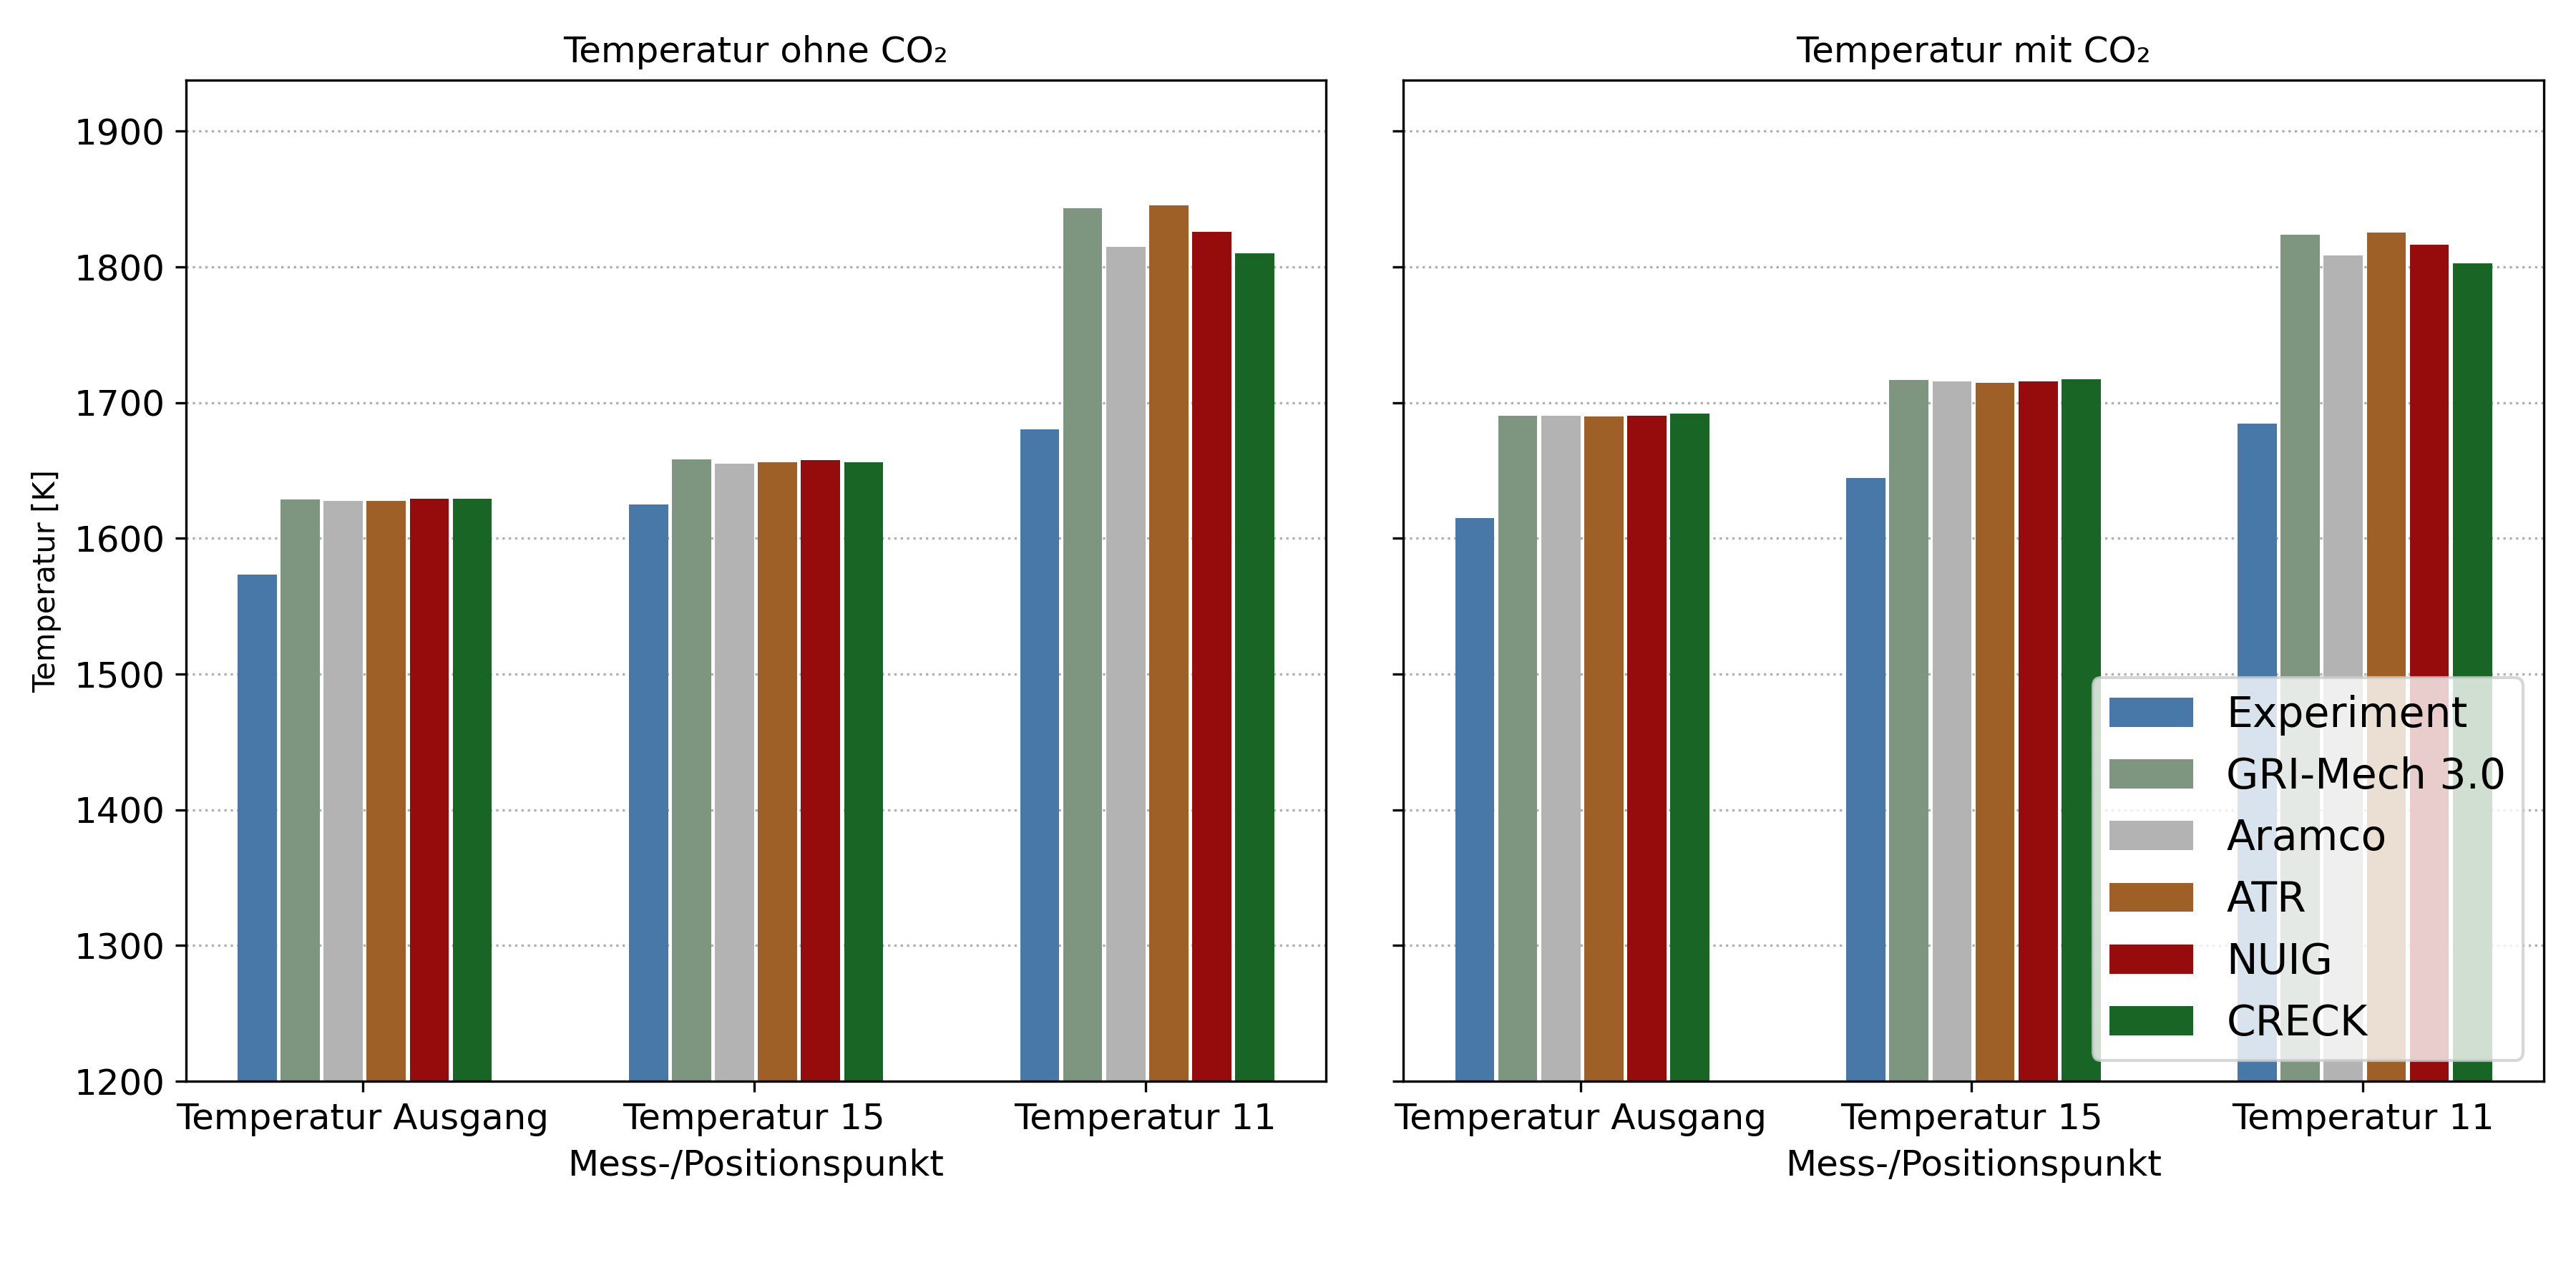
\includegraphics[width=1\linewidth]{img/Vergleich_mech/Vergleich_Temperaturen_gap_manual.png}
            \caption{Vergleich der Temperaturen anhand der Berechnungen verschiedener $\mbox{Reaktionsmechanismen}$ mit experimentellen Daten}
            \label{fig:auswertung_vergleich_exp_temp}
        \end{figure}
        %Auch hier zeigt sich ein ähnliches Verhalten. Fast alle Mechanismen liegen nah beieinander. Ausschließlich der CRECK-Mechanismus weist eine deutliche Abweichung im Fall von zusätzlichem CO$_2$ im Feed auf. Dabei entsprechen die Ergebnisse des CRECK-Mechanismus im Fall 2 am ehesten den gemessenen Temperaturwerten. 

        In beiden Fällen zeigen die Simulationen ein ähnliches Temperaturverhalten mit nur geringen Abweichungen zwischen den Mechanismen. Die größten Differenzen treten am Messpunkt Temperatur 11 auf, wo alle Mechanismen die experimentellen Werte deutlich überschätzen. Während die Ausgangstemperaturen und die Werte am Messpunkt 15 nahezu übereinstimmen, liefern die Mechanismen Aramco und CRECK am Messpunkt 11 die niedrigsten und damit realistischsten Temperaturen.
        %Ohne CO$_2$ (linke Abbildung) liefern GRI-Mech~3.0 und Aramco die besten Übereinstimmungen mit dem Experiment, während CRECK leicht niedrigere Temperaturen berechnet. Mit CO$_2$-Zugabe (rechte Abbildung) verhalten sich die Mechanismen ähnlich, doch der CRECK-Mechanismus liegt hier am nächsten an den gemessenen Temperaturen und bildet den Verlauf insgesamt am realistischsten ab.


        Eine Betrachtung des MSE analog \ref{tab:auswertung_mse_mechanismen} ist hierbei nicht zielführend. Da Temperatur und Stoffmengenanteile verschiedene Größenordnungen besitzen, führt ein einfacher MSE zu einer überproportionalen Betrachtung der Temperaturunterschiede. Ein gewichteter MSE könnte hierbei sinnvolle Vergleichsergebnisse schaffen, die empirische Wichtung muss allerdings validiert werden.

        Da sich alle Temperaturen in einer vergleichbaren Größenordnung bewegen, ist die Betrachtung der Abweichungen in dem Produktgas entscheidender als die Abweichungen der Temperaturen. 

        Aufgrund der Literaturrecherche (vgl. Abschnitt \ref{sec:reaktionsmechanismen_literatur}), der Modellkomplexität und der Ergebnisse in Tabelle \ref{tab:auswertung_mse_mechanismen} wurde Aramco als Mechanismus für die weitere Verwendung ausgewählt. Dieser stellt dabei einen guten Kompromiss aus Rechenzeit, Genauigkeit und Stabilität dar. 
        Für eine ausschließliche Betrachtung des Referenzfalls wäre auch der Einsatz des CRECK-Mechanismus denkbar. Aufgrund seiner höheren Abweichungen im Fall mit CO$_2$-Zugabe wird seine Verwendung jedoch nicht bevorzugt, er kann jedoch als möglicher Alternativmechanismus herangezogen werden.
\iffalse
        Da alle Simulationen mit den verschiedenen Reaktionsmechanismen in einem Identischen Reaktornetzwerk unter konstanten Bedingungen durchgeführt wurden, ist ein Vergleich der Gaszusammensetzungen in der Reforming Zone möglich. In Abbildung \ref{fig:auswertung_verläufe_mechanismen_keinco2} sind diese Zusammensetzungen für den Fall, dass kein zusätzliches CO$_2$ dem Feed zugegeben wird, dargestellt. 
        \begin{figure}[H]
            \centering
            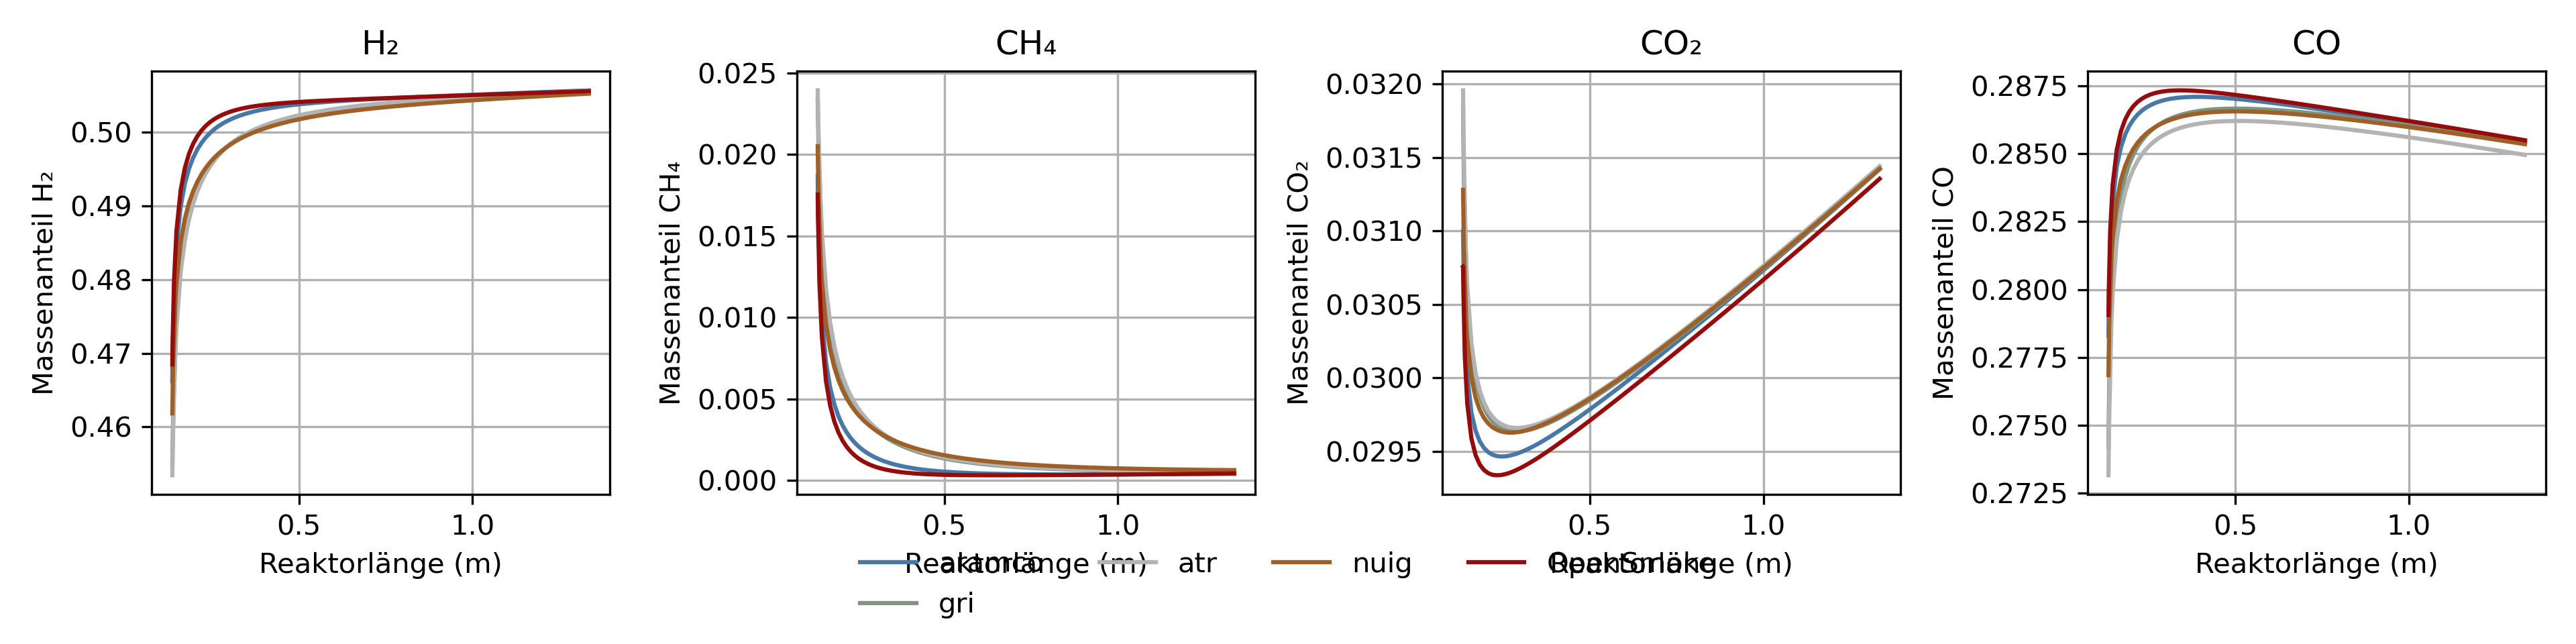
\includegraphics[width=1\linewidth]{img/Vergleich_mech/H2_CH4_CO_CO2_keinCO2.png}
            \caption{Vergleich der Massenprofile der Spezies CO, CO$_2$, H$_2$ und CH$_4$ entlang der Strömungszone anhand der Berechnungen verschiedener $\mbox{Reaktionsmechanismen}$}
            \label{fig:auswertung_verläufe_mechanismen_keinco2}
        \end{figure}
        In Abbildung \ref{fig:auswertung_verläufe_mechanismen_keinco2} kann man gut erkennen, dass es zwar am Anfang des Reaktors signifikante Abweichungen voneinander gibt, während zum Ende des Reaktors kaum Abweichungen vorliegen. Die Abweichung am Anfang des PFRs ist durch die in der Literatur festgestellten Unterschiede im Zündverhalten der Mechanismen begründbar. Die Annäherung zu einem ähnlichen Ergebnis aller Mechanismen ist dadurch begründbar, da sich die Zusammensetzungen in der Nachbrennzone zunehmend dem thermodynamischen Gleichgewicht annähern, wodurch die Unterschiede zwischen den Mechanismen geringer werden.

        \alert{Ein vergleichbares Verhalten der Mechanismen kann auch für den zweiten Fall festgestellt werden}
        \begin{figure}[H]
            \centering
            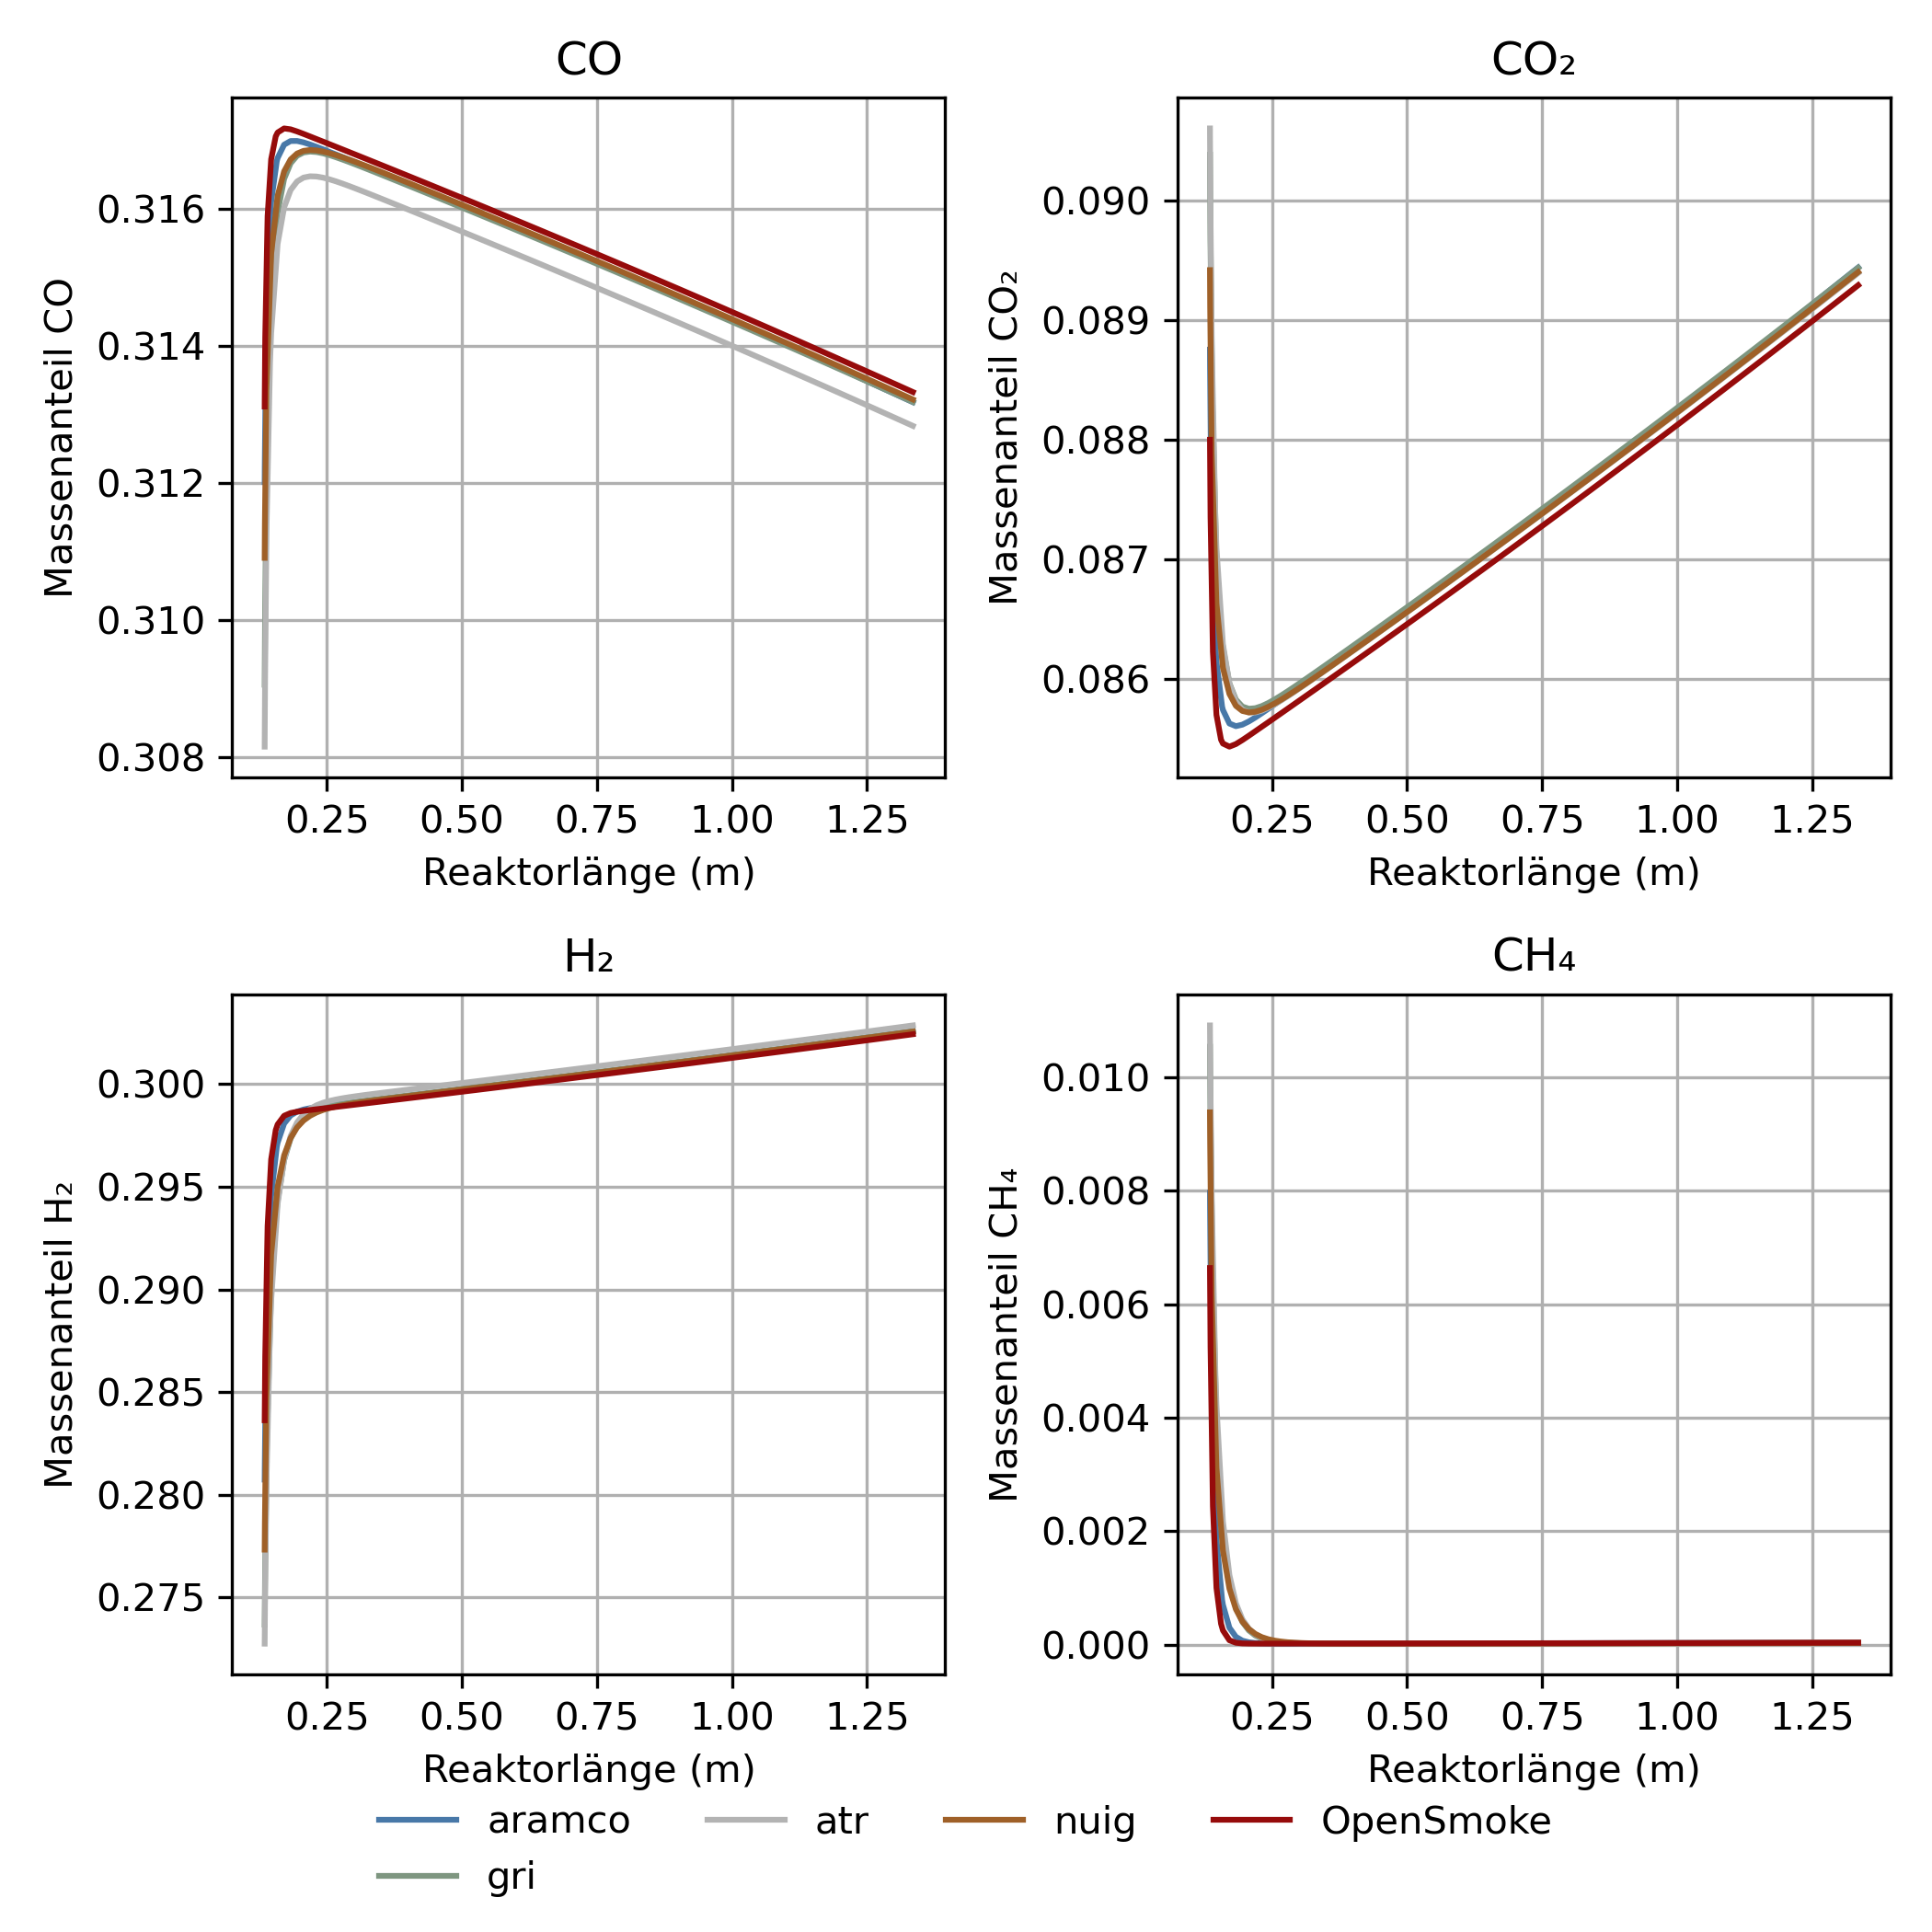
\includegraphics[width=0.6\linewidth]{img/Vergleich_mech/H2_CH4_CO_CO2.png}
            \caption{Vergleich der Massenprofile der Spezies CO, CO$_2$, H$_2$ und CH$_4$ entlang der Strömungszone anhand der Berechnungen verschiedener $\mbox{Reaktionsmechanismen}$}
            \label{fig:auswertung_verläufe_mechanismen_keinco2}
        \end{figure}

        Insgesamt ist die Abweichung der simulierten Ergebnisse im Vergleich zu den gemessenen Werten extrem klein. In Tabelle \ref{tab:auswertung_mse_mechanismen} ist der mittlere quadratische Fehler aller Reaktionsmechanismen für beide Simulationsfälle dargestellt. Die Vollständigen Tabellen aller Fehler für jede Spezies befinden sich im Anhang.
        \begin{table}[H]
            \centering
            \caption{Gesamtfehler (mittlerer quadratischer Fehler, MSE) der betrachteten Reaktionsmechanismen für beide Betriebsweisen}
            \label{tab:auswertung_mse_mechanismene}
            \begin{tabular}{lcc}
                \toprule
                \textbf{Mechanismus} & \textbf{Gesamt-MSE (kein CO$_2$)} & \textbf{Gesamt-MSE (mit CO$_2$)} \\
                \midrule
                GRI-Mech 3.0   & 0{,}00006 & 0{,}00023 \\
                Aramco         & 0{,}00004 & 0{,}00026 \\
                ATR-Mechanismus & 0{,}00006 & 0{,}00023 \\
                NUIG           & 0{,}00004 & 0{,}00022 \\
                Smoke          & 0{,}00003 & 0{,}00029 \\
                \bottomrule
            \end{tabular}
        \end{table}
        Bemerkenswert ist jedoch, dass die Ergebnisse bei der Simulation mit CO$_2$-Zugabe um ein vielfaches höher sind als bei der Referenzvariante. Dadurch, dass diese Reaktionsmechanismen ursprünglichen für die Anwendung der Verbrennung entwickelt wurden, sind die CO$_2$-haltigen Gleichgewichte (u.a. Wassergas-Shift-Reaktion) nicht optimal parametrisiert, da diese bei stöchiometrischer Flammenvalidierung kaum Gewicht haben.
        %Eine Mögliche Erklärung für diese Beobachtung ist, dass die Gleichgewichtsreaktionen, die CO$_2$ beinhalten, in der ursprünglichen Anwendung weniger Relevanz hatten, und diese dadurch weniger exakte Reaktionsparameter vorweisen. 

        Insgesamt stützt diese Auswertung dabei die These, dass alle Reaktionsmechanismen eine gute Genauigkeit aufweisen und erklärt ebenfalls die verschiedenen Ergebnisse verschiedener Studien. Demnach ist die Auswahl des passendsten Mechanismus immer eine Frage der Prozessbedingungen und der beste Mechanismus kann ohne Vorbetrachtungen nicht explizit erkannt werden. Beispielsweise ist in den Ergebnissen dieses Vergleiches der Fehler des CRECK-Mechanismus in einem Fall klein, in dem anderen Fall verhältnismäßig groß.

        Darüber hinaus zeigen die sehr kleinen Fehler zudem, dass es bei der Wahl des geeigneten Mechanismus vielmehr auf die Art der geforderten Reaktionen und die Effizienz der Berechnungen ankommt als auf die eigentlichen kinetischen Parameter der Studien, da diese in vielen Fällen ähnliche Ergebnisse liefern. 

        Obwohl der Aramco-Mechanismus im Fall der CO$_2$-unterstützten POx etwas größere Abweichungen aufweist als andere Mechanismen, wird er für die folgenden Simulationen dieser Arbeit verwendet. Ausschlaggebend hierfür ist der, wie zuvor beschrieben, gute Kompromiss aus Genauigkeit, Detaillierungsgrad, numerischer Stabilität und Recheneffizienz. Darüber hinaus wird der Aramco-Mechanismus in der Literatur häufig als Referenzmechanismus herangezogen, wodurch er sich besonders für vergleichende Studien und die Untersuchung unterschiedlicher Prozessbedingungen eignet.
\fi 
    \section{Erweiterungen des Reaktornetzwerkmodells}
        Bis zu diesem Zeitpunkt wurde für alle Simulationen ein linear aufgebautes Reaktornetzwerk, bestehend aus einem PSR und einem PFR, genutzt. Da jedoch aufgrund einer CFD-Analyse (siehe Kapitel \ref{sec:vorbetrachtungen}) bekannt ist, dass der Reaktor ein anderes Strömungsverhalten aufweist, wurde mithilfe weiterer Reaktoren das Reaktornetzwerk erweitert, um die Bedingungen im Reaktor besser abbilden zu können.

        Da in den Reaktornetzwerken keine vergleichbaren PFRs mehr enthalten sind, ist eine Auswertung der Profile dieser Reaktoren kaum noch möglich und der Vergleich dieser Netzwerke bezieht sich allein auf die Produktgaszusammensetzung. In Abbildung \ref{fig:auswertung_erweiterungen_spezies} sind diese Produktgaszusammensetzungen dargestellt. 
        \begin{figure}[H]
            \centering
            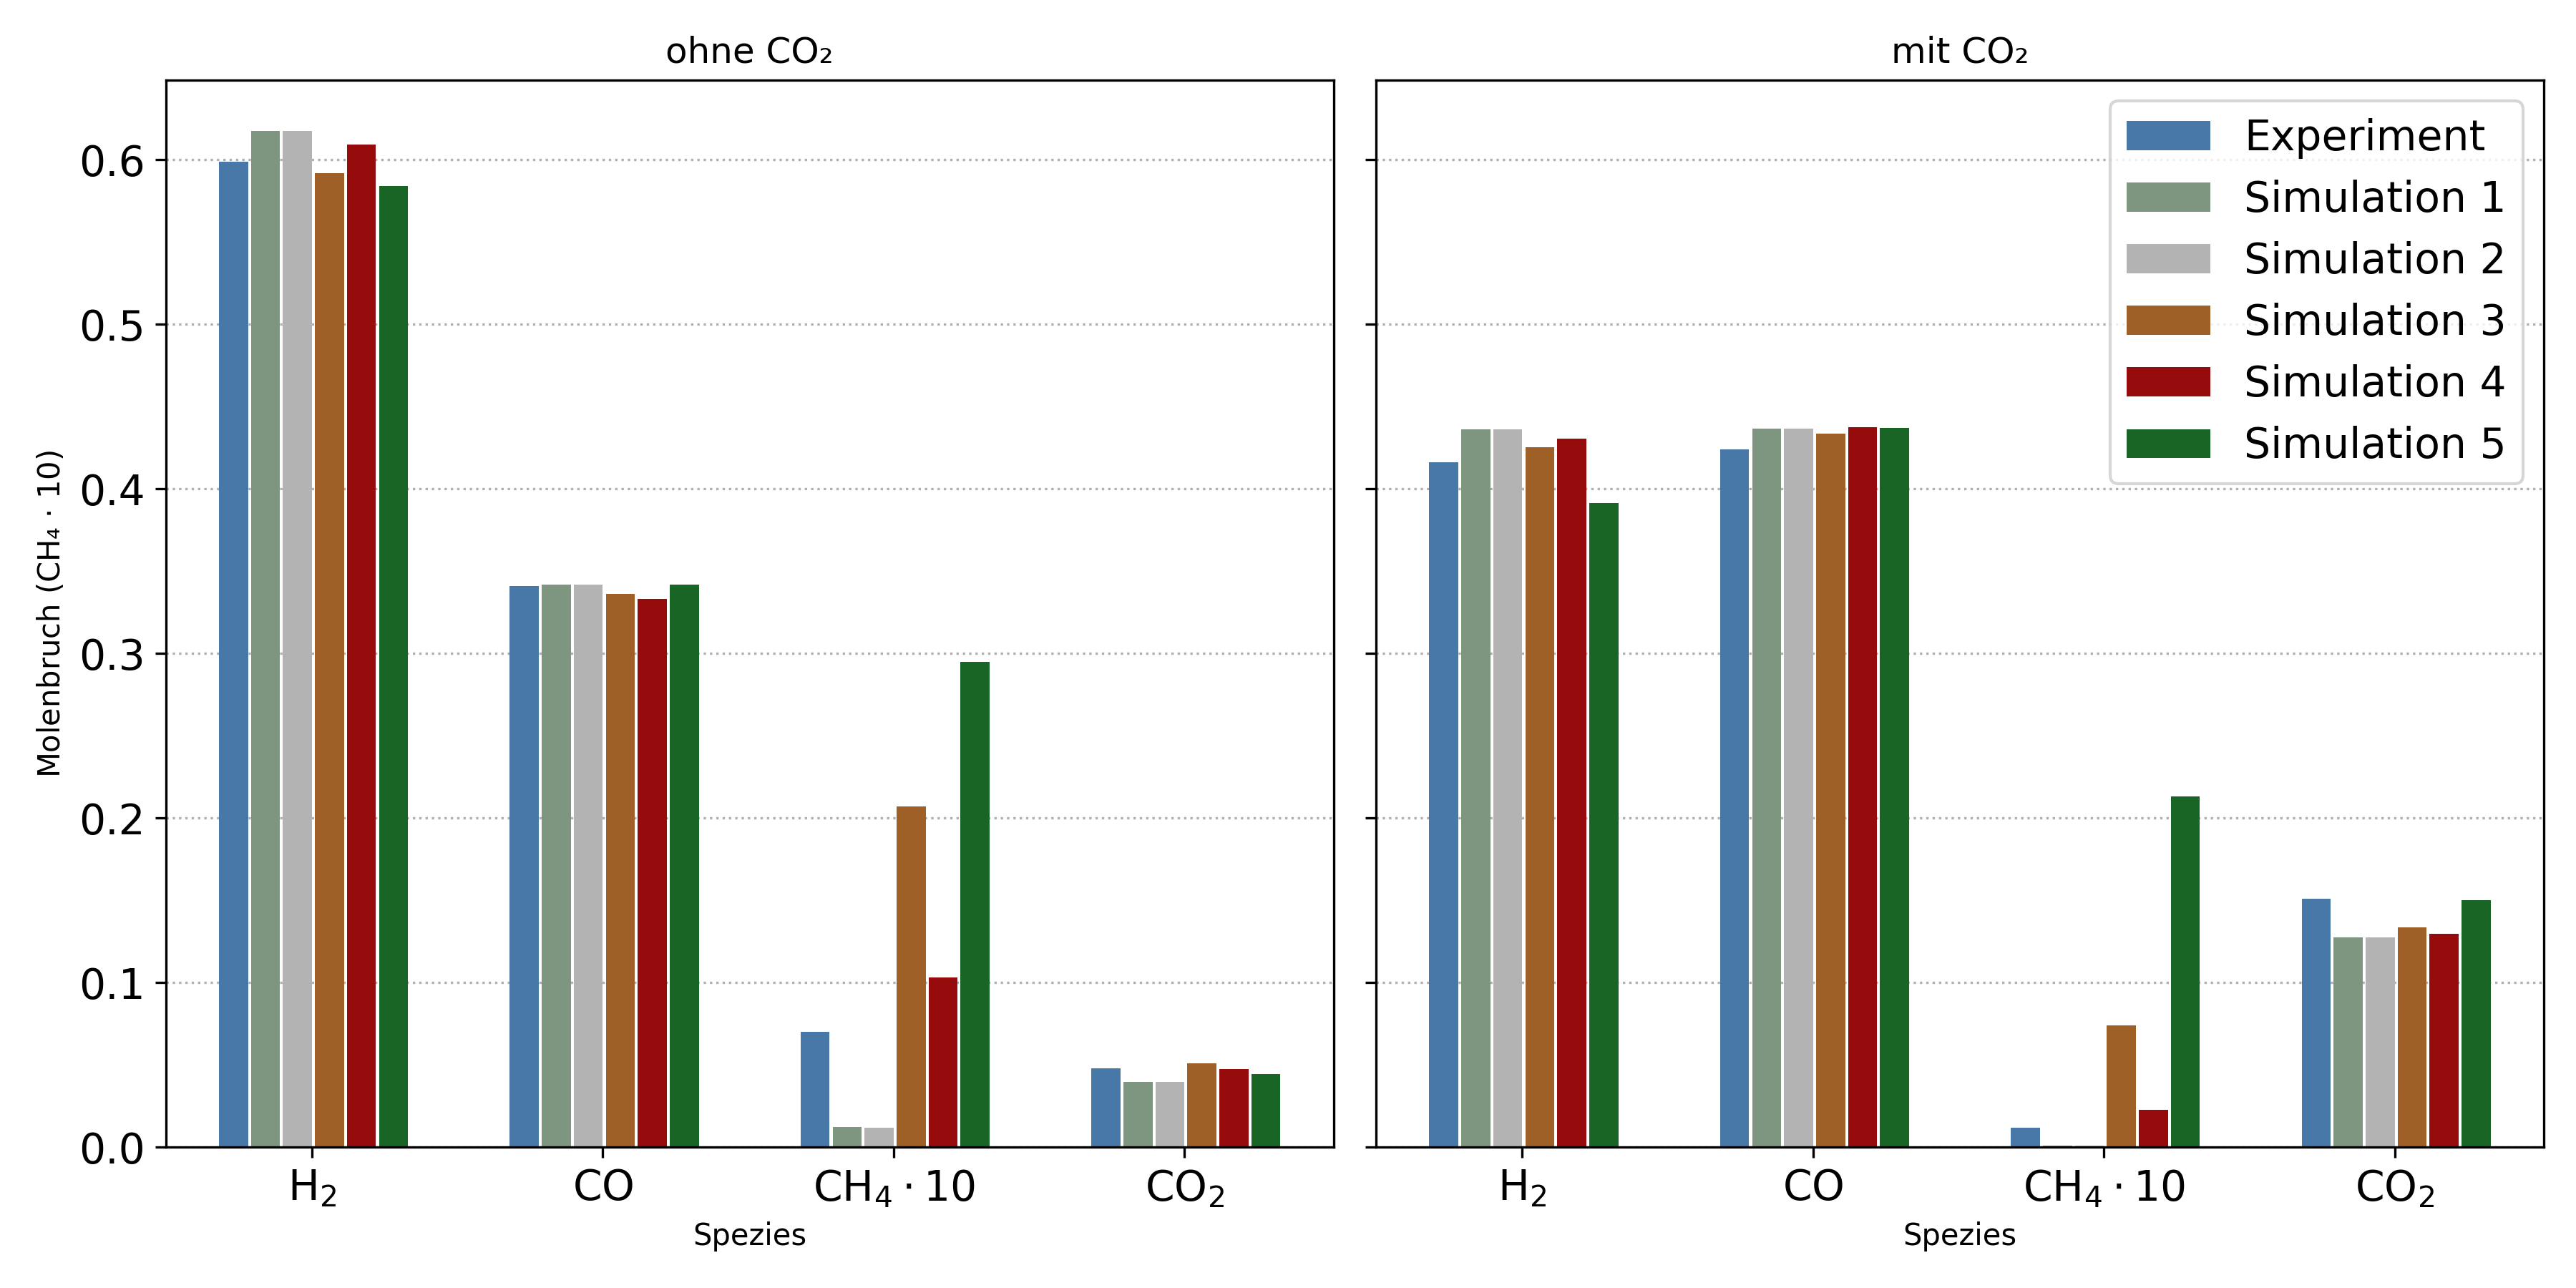
\includegraphics[width=1\linewidth]{img/Erweiterungen/Vergleich_Erweiterungen.png}
            \caption{Gemessene und simulierte Produktgaszusammensetzung verschiede\-ner Reaktornetzwerke}
            \label{fig:auswertung_erweiterungen_spezies}
        \end{figure}
        Um die verschiedenen Netzwerke untereinander zu vergleichen wird wieder der mit\-tlere quadratische Fehler zwischen den Simulationen ermittelt. Dieser ist in Tabelle \ref{tab:tvd_modelle} dargestellt.
        \begin{table}[H]
            \centering
            \caption{Berechneter mittlerer quadratische Fehler (MSE) der Modelle mit und ohne CO$_2$}
            \label{tab:tvd_modelle}
            \begin{tabular}{lcc}
                \toprule
                \textbf{Modell} & \textbf{MSE (ohne CO$_2$)} & \textbf{MSE (mit CO$_2$)} \\
                \midrule
                1 & 0,00011 & 0,00028 \\
                2 & 0,00011 & 0,00028 \\
                3 & 0,00007 & \textbf{0,00013} \\
                4 & \textbf{0,00004} & 0,00021 \\
                5 & 0,00018 & 0,00029 \\
                \bottomrule
            \end{tabular}
        \end{table}
        Man kann erkennen, dass es keine kontinuierliche Verbesserung der Modelle gibt. Das komplexeste Rechenmodell weist dabei sogar den größten Fehler mit einer sehr großen Überschätzung des Methanaustritts auf. Wie in Kapitel \ref{sec:auswertung_mechanismus} bereits erläutert, sind die Abweichungen größer, wenn zusätzlich zum Referenz-POx-Prozess noch Kohlenstoffdioxid hinzugegeben wird. Dies kann in jedem Modell festgestellt werden. Aus Tabelle~\ref{tab:tvd_modelle} geht hervor, dass im zweiten Fall Modell~3 die geringste Gesamtabweichung liefert, obwohl in Abbildung~\ref{fig:auswertung_erweiterungen_spezies} erkennbar ist, dass der Methanschlupf von Modell~4 näher am experimentellen Wert liegt. Da die Methankonzentrationen sehr gering sind, wirkt sich diese Abweichung insgesamt nur geringfügig auf die Gesamtbewertung aus.

        Zwischen Modell 1 und Modell 2 können keine Veränderungen in der Abweichung festgestellt werden. Da sich Modell 2 um einen hinzugefügten Bypass von Modell 1 unterscheidet, ergibt sich die Beobachtung, dass der Stoffstrom im Bypass keine Auswirkungen auf die Reaktionsbedingungen hat. Da im Bypass kein Sauerstoff als Reaktionspartner vorhanden ist, wird das Methan dementsprechend nicht im Bypass, sondern in der Nachbrennzone umgesetzt. Dabei kommen folgende Reaktionen neben Radikalbildungen infrage:
        \begin{align}
            \mathrm{CH_4 + H_2O} & \leftrightharpoons\mathrm{ CO + 3\ H_2} \\ 
            \mathrm{CH_4 + CO_2} & \leftrightharpoons \mathrm{2\ CO +2\ H_2}
        \end{align}
        Diese endothermen Reaktionen laufen in der Nachbrennzone aufgrund der dort vorherrschenden hohen Temperaturen trotz ihrer kinetischen Trägheit mit hinreichender Geschwindigkeit ab und tragen somit zusätzlich zum Abbau des Methans bei.

        Eine Erweiterung dieses Modells mit einem PSR als Rezirkulationszone sorgt für eine höhere Genauigkeit beider Simulationsfälle. So ergibt sich bei dem Fall mit CO$_2$ das genaueste Modell, während es im Referenzfall das zweitbeste Modell darstellt. Insgesamt überschätzt dieses Modell den Schlupf von Methan deutlich, stellt dafür die Komponenten Wasserstoff, Kohlenstoffmonoxid und Kohlenstoffdioxid gut dar. Die Rückführung des bereits entstandenen Produktgases durch die Rezirkulationszone sorgt zwar für eine höhere Temperatur in dem Bypass, verdünnt aber gleichzeitig noch nicht umgesetztes Methan, weshalb sich der zu hohe Schlupf von Methan ergibt. 

        Wenn die Rezirkulationszone stärker im Austausch mit der Nachbrennzone steht, was durch Reaktornetzwerk 4 umgesetzt wurde, indem ein zusätzlicher Strom durch die Teilung des PFRs hinzugefügt wurde, wird die Umsetzung des Methans durch beide Simulationen am genauesten berechnet. Insgesamt ist dieses reduzierte Modell am besten geeignet, um die herkömmliche POx ohne Zugabe von CO$_2$ im Feed zu modellieren. Auch im zweiten Fall wird eine hohe Genauigkeit erreicht, allerdings mit weniger Übereinstimmung als mit dem vorherigen Modell. 

        Durch die Auftrennung des PFRs wird ein Teil des entstandenen Produktgases zurück in die Bypasszone geführt. Dadurch wird noch nicht umgesetztes Methan mit Restbeständen Sauerstoff aus dem Produktgas in Verbindung gebracht, und noch nicht umgesetztes Methan im PFR wird erneut durch den Reaktor geleitet. Insgesamt ist somit eine Abschätzung der Produktgaszusammensetzung möglich. Da in diesem Modell die Interaktion mit der Rezirkulationszone erweitert wurde, spielen chemische Gleichgewichte eine größere Rolle. Da diese im Fall der trockenen Reformierung größere Fehler aufweisen, kann die geringere Genauigkeit des CO$_2$-Falls erklärt werden. 

        Durch die Auftrennung der Rezirkulationszone in zwei Teile, sowie die umfangreiche Interaktion beider Zonen mit der Strömungszone, entsteht das in dieser Arbeit komplexeste Modell. Die Modellierung mit diesem Modell führt zu den größten Abweichungen aller Modelle. Insbesondere der Schlupf von Methan wird deutlich überschätzt.

        Aufgrund der hohen Komplexität des Modells durch zwei getrennte Rezirkulationszonen und viele Interaktionen der Reaktoren untereinander, sind im Vergleich zu den einfacheren Modellen deutlich mehr Annahmen zu treffen. Dadurch, dass die einfacheren Modelle sehr genaue Ergebnisse liefern, hat die große Anzahl an getroffenen Annahmen einen insgesamt negativen Effekt auf die Modellgüte. Darunter befindet sich die Aufteilung der Ströme und die Größen der Reaktoren. Eine Trennung der Rezirkulationszone kann sich zudem negativ auf den Wärmeübergang in dem Reaktor auswirken. Ein sehr komplexes Modell hat zudem starken Einfluss auf die Rechenzeit und numerische Stabilität. 

        In Abbildung \ref{fig:auswertung_erweiterungen_temperaturen} sind die simulierten Temperaturen dargestellt. 
        \begin{figure}[H]
            \centering
            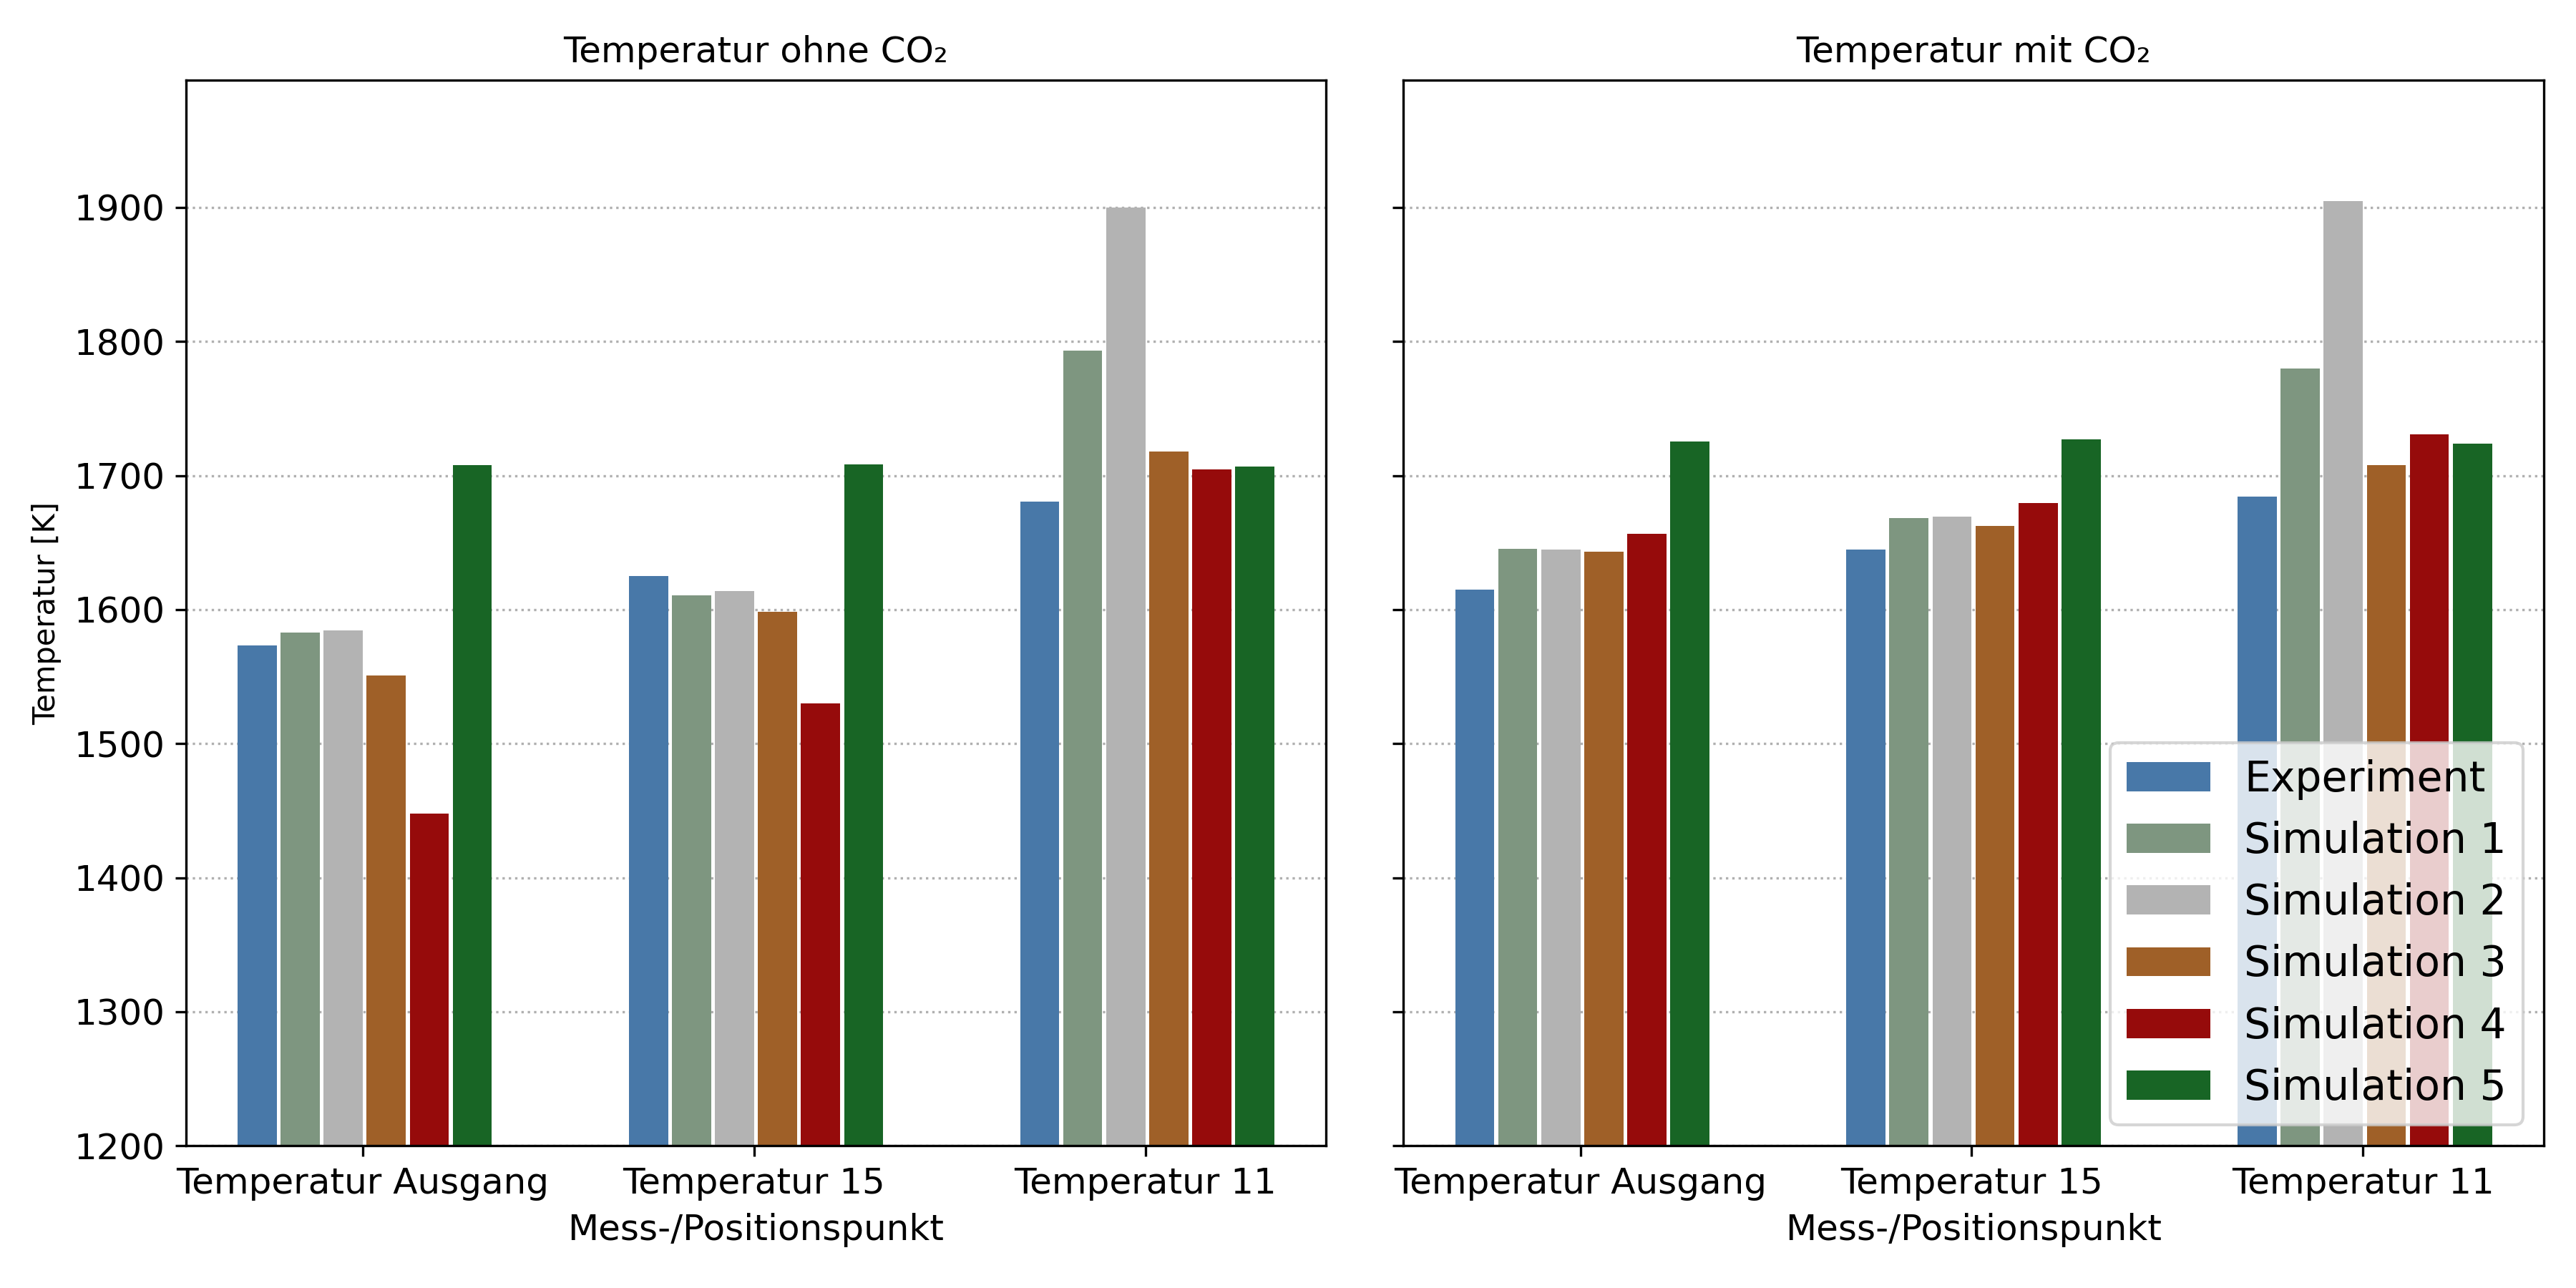
\includegraphics[width=1\linewidth]{img/Erweiterungen/Vergleich_Temperaturen.png}
            \caption{Gemessene und simulierte Temperaturen verschiede\-ner Reaktornetzwerke}
            \label{fig:auswertung_erweiterungen_temperaturen}
        \end{figure}
        Hierbei befinden sich alle Temperaturen in einer ähnlichen Größenordnung. Dabei weist das komplexeste Modell wieder von den Experimentaldaten aufgrund nicht optimalen Modellannahmen ab.
    \section{Rechenzeit}
        Damit umfangreiche Parameterstudien durchgeführt werden können, ist eine kurze Rechenzeit von hoher Bedeutung. Während Reaktornetzwerkmodell~1 eine Rechenzeit von etwa 7~s und Reaktornetzwerkmodell~2 eine Rechenzeit von etwa 14~s aufweist, beträgt die Rechenzeit der Modelle mit Rückkopplung über 10~Minuten. In Tabelle \ref{tab:rechendauer} sind die Rechenzeiten der Modelle aufgelistet. Dabei gab es keine Unterschiede bei der Berechnung beider Fälle.
        \begin{table}[H]
            \centering
            \caption{Übersicht über die gemessene Rechendauer der verschiedenen Reaktormodelle}
            \begin{tabular}{c c}
                 \toprule
                 Modell & Rechenzeit in Sekunden \\
                 \midrule
                 1 & 7 \\
                 2 & 14 \\ 
                 3 & 630 \\ 
                 4 & 720 \\ 
                 5 & 750 \\
                 \bottomrule
            \end{tabular}
            \label{tab:rechendauer}
        \end{table}
        Da die Rechenzeit nicht nur von der Modellkomplexität, sondern auch von der genutzten Hardware, getroffenen Abschätzungen, numerischen Einstellungen und vielen anderen Faktoren abhängig ist, dient diese Übersicht nicht als klare Angabe der Rechenzeit, sondern vielmehr zur Darstellung eines Trends. 

        Es ist erkennbar, dass die linearen Modelle sehr schnelle Lösungen ergeben, da diese keine iterative Lösung aufweisen. Durch die Iteration ab Modell 3 ergeben sich deutlich höhere Rechenzeiten. Eine Abweichung zwischen Modell~4 und 5 ist kaum zu erkennen, da die Berechnung eines einzelnen PSRs kaum Rechenzeit in Anspruch nimmt. 
        
        Durch den damit verbundenen deutlich höheren Rechenaufwand sind diese kom\-plexeren Modelle nur eingeschränkt für Parameterstudien geeignet. Aufgrund der hohen Modellgüte der einfachen Netzwerke ist es daher sinnvoller, die Parameterstudien mit einem dieser Modelle durchzuführen. Soll ein höherer Detailgrad der Ergebnisse erzielt werden, können im Anschluss auf Basis der Parameterstudie gezielte Einzelsimulationen mit komplexeren Reaktornetzwerken erfolgen. Zwar kann durch eine Anpassung der Lösungsparameter sowie der numerischen Dämpfung eine Beschleunigung der Berechnung erreicht werden, da die optimalen Parameter jedoch stark von den Prozessbedingungen abhängen, ist dieser Ansatz im Rahmen einer Parameterstudie nicht relevant. Eine signifikante Abweichung der Rechenzeiten der Modelle~3 bis 5 konnte nicht festgestellt werden, da der überwiegende Teil der Rechenzeit durch die iterative Annäherung an den stationären Zustand bestimmt wird, was bei allen Modellen einen vergleichbaren Aufwand verursacht. Zudem ist die Lösung des zusätzlich eingefügten PSRs im Vergleich zu den bereits vorhandenen PFRs deutlich weniger rechenintensiv, wodurch sich der Gesamtaufwand nur geringfügig verändert.
    \section{Parameterstudie CO$_\mathbf 2$}
        Ziel des Projekts \textit{SCOORE} ist die Entwicklung neuer Prozesse zum Recycling bzw. Nutzen von Kohlenstoffdioxid \cite{Scoore_Enargus}. Damit der Prozess sowohl das Recycling von CO$_2$ ermöglichen soll, als auch wirtschaftlich und produktionstechnisch in Produktionsketten integriert werden kann, ist eine Parameterstudie zum Untersuchen des CO$_2$-Feedmassen\-stroms essentiell.

        Da in den vorherigen Kapiteln bereits gezeigt wurde, dass ein lineares Reaktornetzwerk eine ausreichend hohe Genauigkeit bei geringer Rechendauer liefert, wird dieses Modell für die nachfolgende Parameterstudie verwendet. Aufgrund der geringen Rechenzeit eignet es sich besonders für umfangreiche Simulationsreihen und ermöglicht eine effiziente Untersuchung der relevanten Einflussgrößen.
        
        %Da in Kapitel \ref{sec:auswertung_mechanismus} festgestellt wurde, dass ein einfaches lineares Reaktornetzwerk ausreicht, um Prozesse mit ausreichend Genauigkeit zu quantifizieren, kann für diese Parameterstudie auf dieses einfache Reaktornetzwerk zurückgegriffen werden, um effizient eine Parameterstudie durchzuführen. 

        Da der eingesetzte Rohstoff Methan (bzw. Erdgas) sowohl kostenintensiv ist, als auch ein hohes Treibhauspotential besitzt, ist es sowohl aus ökologischen und ökonomischen Gründen essentiell, einen Schlupf von Methan zu minimieren. Darüber hinaus ergibt sich ein Grenzwert von 0,5~Vol.-\% aus den Einschränkungen der nachgeschalteten Prozesse, insbesondere der Gasreinigungseinheiten. In Abbildung \ref{fig:auswertung_co2_methanschupf} ist der Methanschlupf in Abhängigkeit des CO$_2$-Massenstroms dargestellt. 
        \begin{figure}[H]
            \centering
            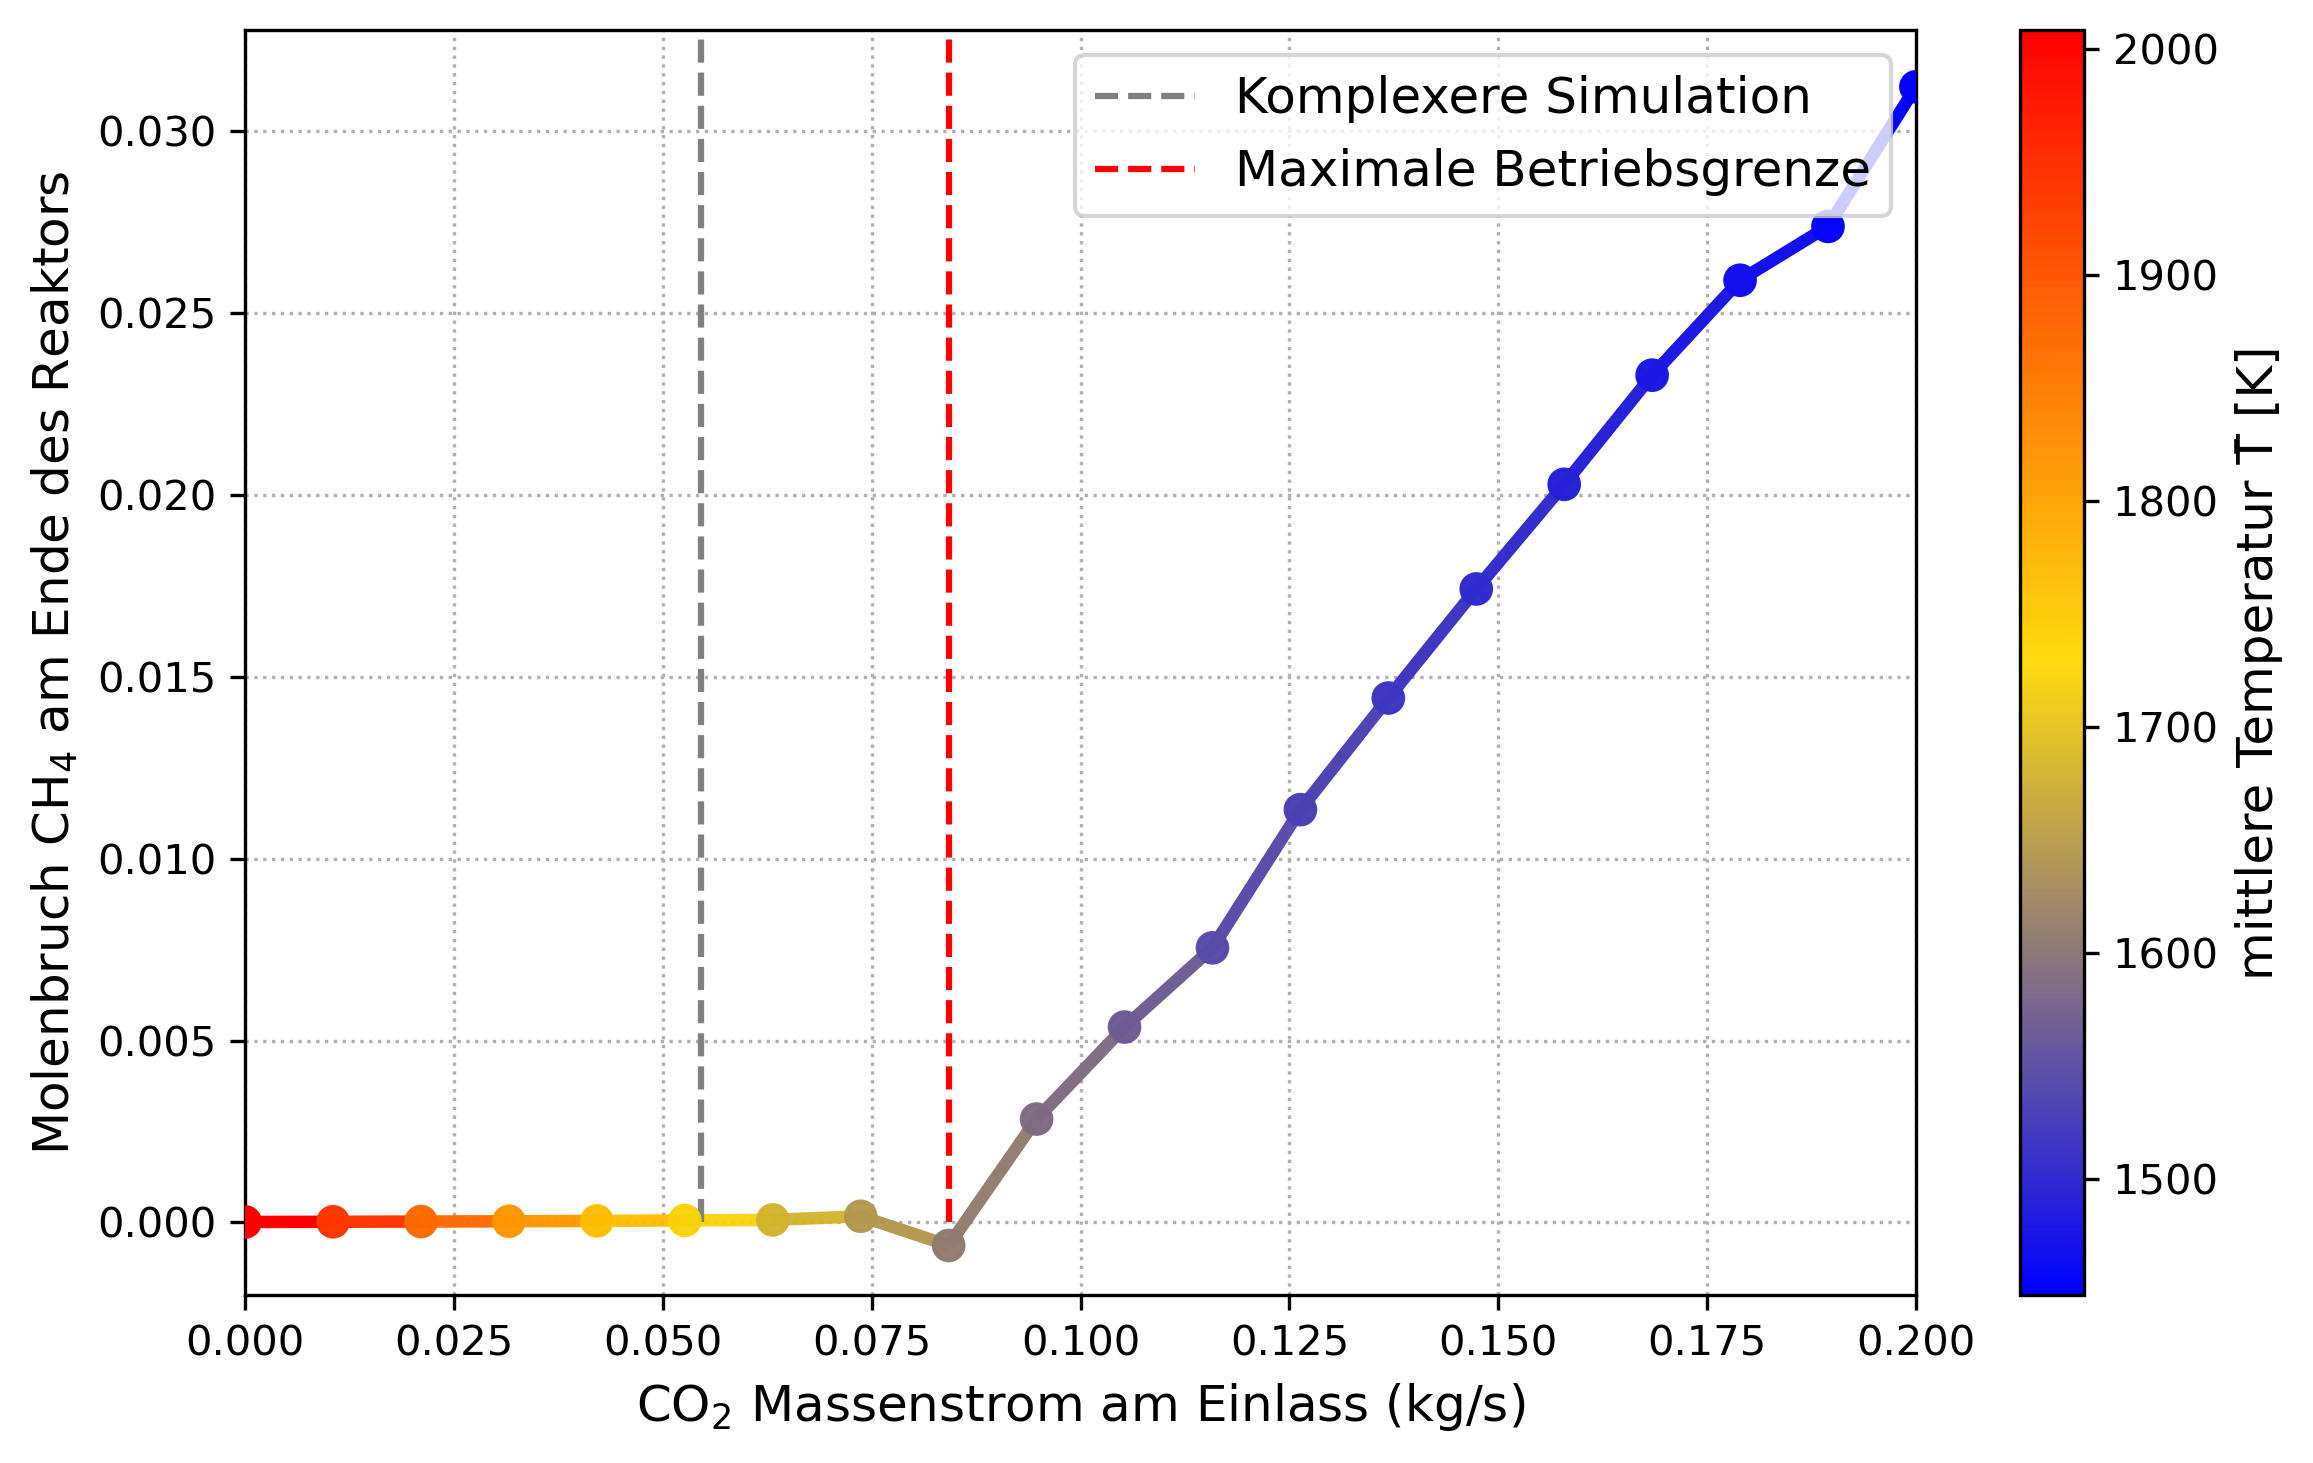
\includegraphics[width=0.75\linewidth]{img/Parameterstudie_CO2/Parameterstudie_CO2_CH4_Schlupf_colormap_marker.png}
            \caption{Methanschlupf und mittlere Temperatur des Reaktors als Ergebnis der Parameterstudie zur Variation des Massenstroms von Kohlenstoffdioxid. Die senkrechte Markierung stellt den Massenstrom im näher betrachteten Fall der POx dar.}
            \label{fig:auswertung_co2_methanschupf}
        \end{figure}
        In Abbbildung \ref{fig:auswertung_co2_methanschupf} ist erkennbar, dass ab einem CO$_2$-Massenstrom von 0,09~kg/s ein linearer Anstieg vorliegt. Dieser lineare Anstieg deutet darauf hin, dass ab dieser Grenze eine erhöhte Zugabe von CO$_2$ eine Umsetzung von Methan direkt verhindert. Dies stellt somit die obere Grenze der Betriebsbedingungen des Reaktors dar. 

        %Dieses Verhalten lässt sich durch mehrere Effekte erklären. Zum einen senkt die Zugabe von CO$_2$ die Temperatur durch eine Erhöhung der Wärmekapazität des Gasgemisches. Gleichzeitig führt eine Verdünnung dazu, dass weniger Sauerstoffmoleküle mit Methanmolekülen reagieren können. Beides sorgt dabei für eine niedrigere Temperatur, wodurch keine vollständige Umsetzung des Methans mehr gegeben ist.

         Dieses Verhalten lässt sich im Wesentlichen durch die Verdünnung des Feeds erklären. Bei Zugabe von Kohlenstoffdioxid muss das umgesetzte Methan eine größere Gasmenge erwärmen, wodurch die Temperatur absinkt. Die niedrigere Temperatur führt wiederum zu einer reduzierten Reaktionsgeschwindigkeit und damit zu einer geringeren Umsetzung von Methan.

        Der erkennbar negative Wert besitzt hierbei keine physikalische Bedeutung, da der Stoffmengenanteil nur Werte im Bereich zwischen 0 und 1 annehmen kann. Diese negativen Werte sind auf numerische Ungenauigkeiten in der Simulation zurückzuführen und entstehen durch Rundungs- und Iterationsfehler bei geringen Konzentrationen. Sie werden daher als numerisches Rauschen interpretiert und auf 0 gesetzt, was einer vollständigen Umsetzung von Methan entspricht. 

        Um sowohl das Ziel der Einsparung von Kohlenstoffdioxidemissionen, als auch die Einbindung in Prozessketten zu ermöglichen, muss ein Betriebspunkt ermittelt werden, bei dem ein hoher Verbrauch von CO$_2$ stattfindet und das Synthesegas ein geeignetes Verhältnisses von Wasserstoff zu Kohlenstoffmonoxid aufweist. Die CO$_2$-Bilanz wird im folgenden als 
        \begin{align}
            X = \frac{\dot m_{out} - \dot m_{in} }{\dot m_{in}} 
        \end{align}
        definiert. Dadurch ergibt sich ein Verbrauch von Kohlenstoffdioxid bei einer negativen Bilanz. In Abbildung \ref{fig:auswertung_co2_bilanz} sind beide beschriebenen Kennzahlen als Ergebnis der Parameterstudie dargestellt. 
        \begin{figure}[H]
            \centering
            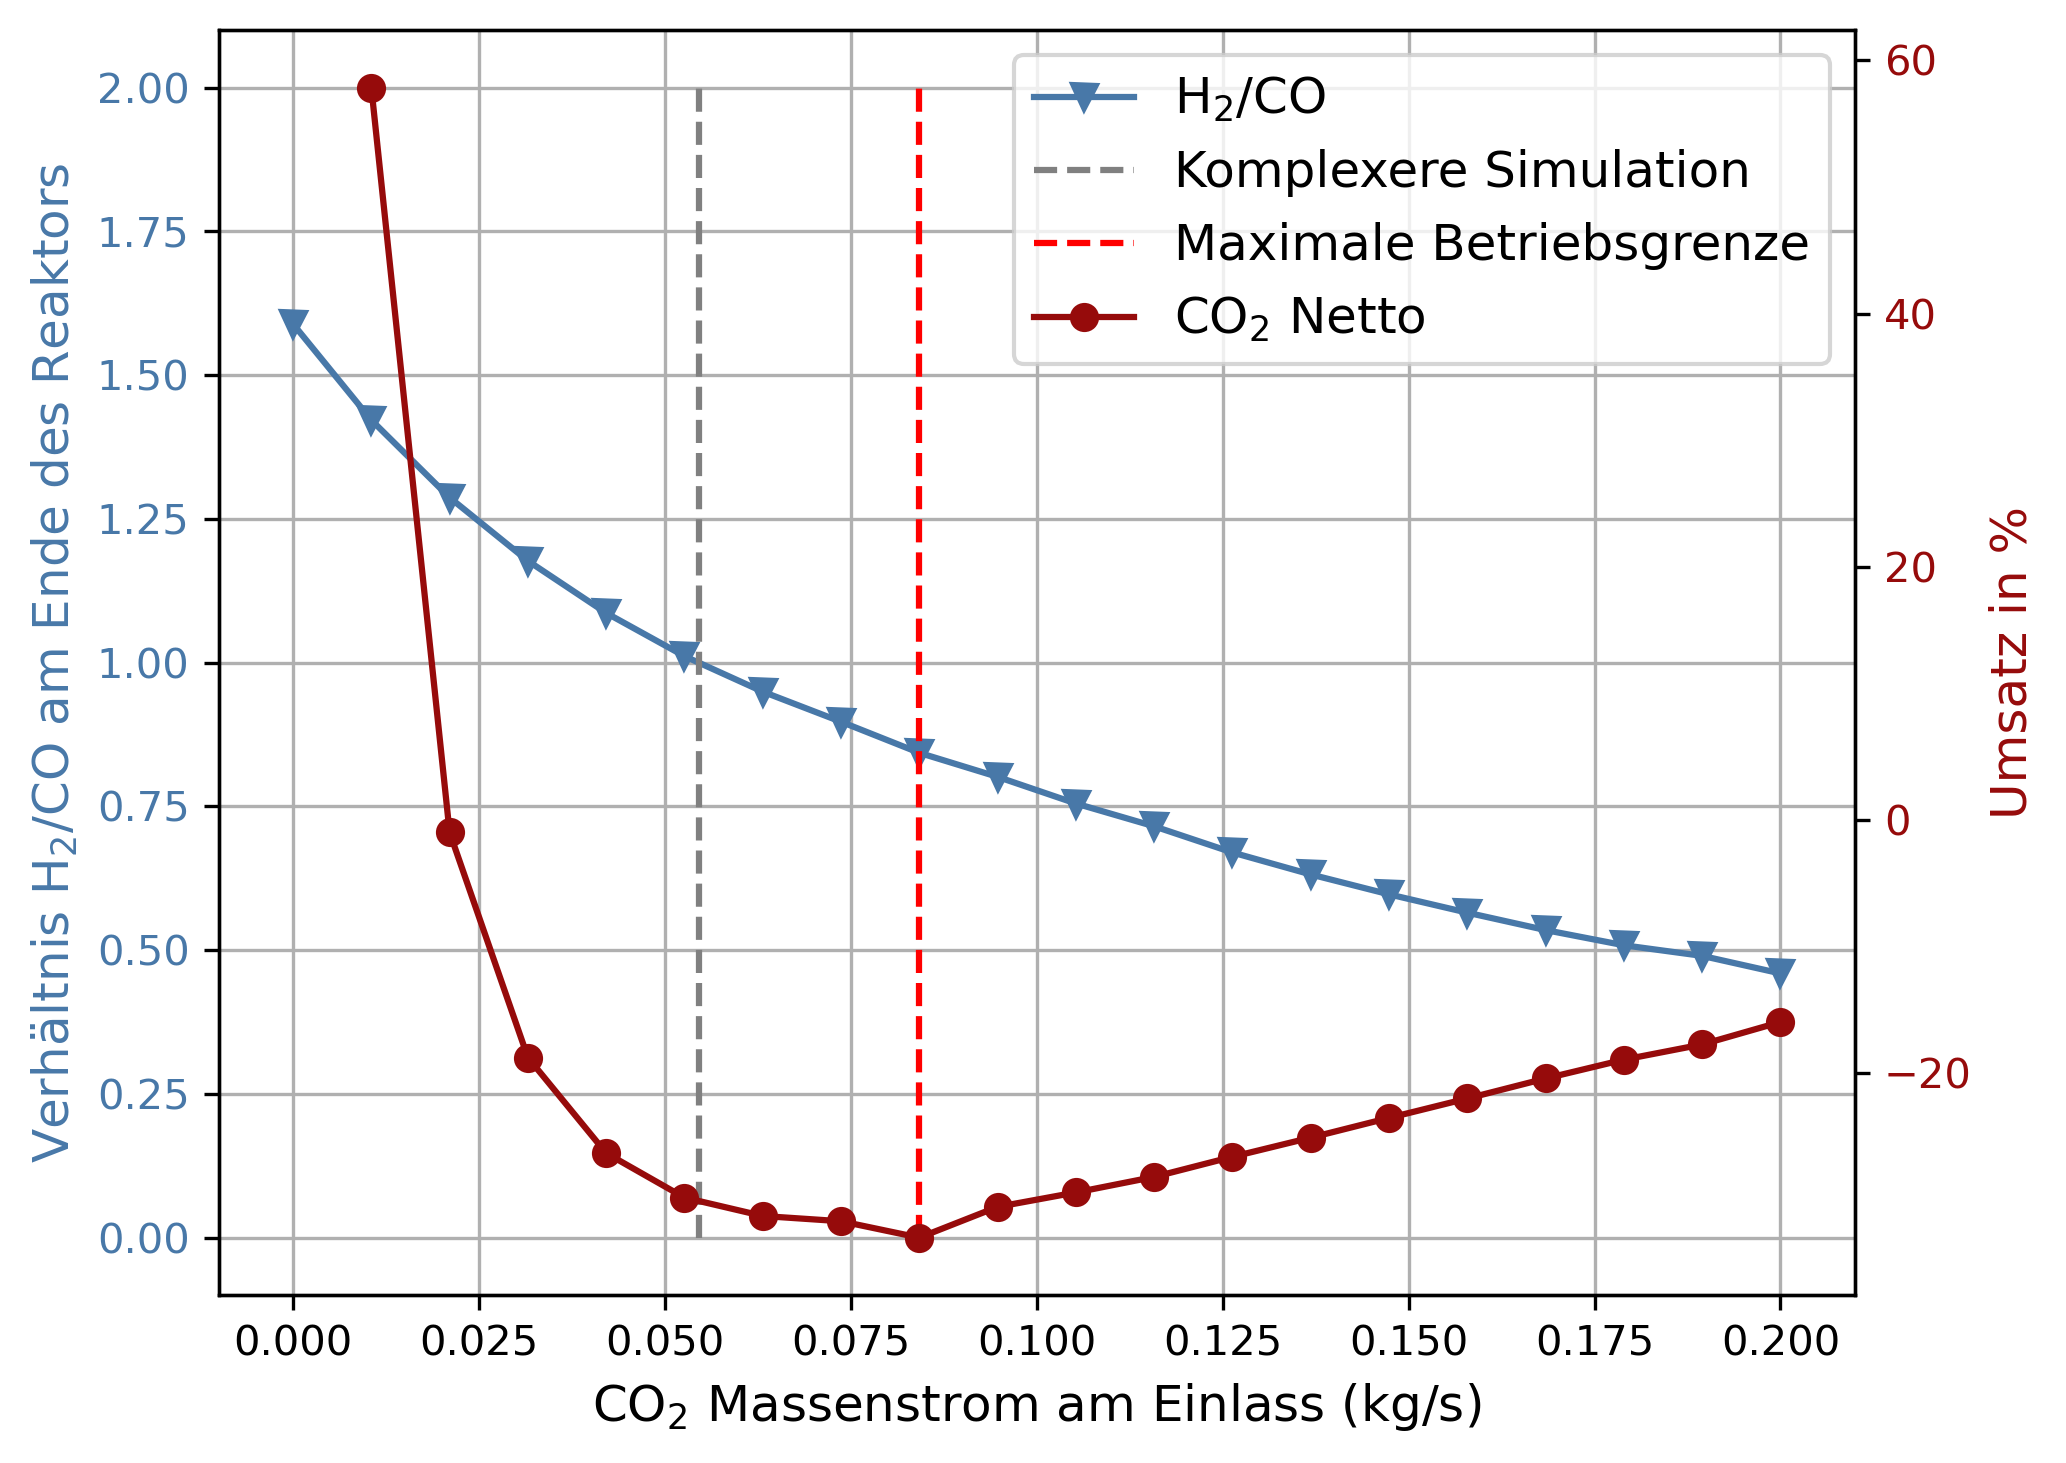
\includegraphics[width=0.75\linewidth]{img/Parameterstudie_CO2/Parameterstudie_CO2_Bilanz.png}
            \caption{CO$_2$-Bilanz und H$_2$/CO-Verhältnis als Ergebnis der Parameterstudie zur Variation des Massenstroms von Kohlenstoffdioxid. Die senkrechte graue Markierung stellt den Massenstrom im näher betrachteten Fall der POx dar}
            \label{fig:auswertung_co2_bilanz}
        \end{figure}
        Mit steigendem Massenstrom steigt der Verbrauch von Kohlenstoffdioxid an, während das H$_2$/CO-Verhältnis kontinuierlich sinkt. Dies ist durch die verstärkte Rückreaktion der Wassergas-Shift-Reaktion erklärbar, da mehr CO$_2$ zu einer Verschiebung des Gleichgewichts führt. Ab der maximalen Betriebsgrenze, ab der das zugeführte Methan nicht mehr vollständig umgesetzt wird, wird auch der Umsatz von Kohlenstoffdioxid geringer. 
        Dieser Trend resultiert aus der Verschiebung des Wassergas-Shift-Gleich\-gewichts in Richtung CO-Bildung.
        \begin{align}
            \mathrm{CO_2 + H_2 \longrightarrow CO + H_2O}
        \end{align}
        Dadurch kommt es sowohl zu einer sinkenden Wasserstoffkonzentration als auch zu einer steigenden Konzentration von Kohlenstoffmonoxid, wodurch sich dieser Trend ergibt. Da für Prozesse wie die Methanolsynthese jedoch Verhältnisse von 2 nötig sind,
        \begin{align}
            \mathrm{CO + 2\ H_2 \longrightarrow CH_3OH}
        \end{align}
        ergibt sich der Bedarf von zusätzlichem Wasserstoff. Die Betriebsparameter aus Tabelle \ref{tab:rahmenbedingungen_versuche} ermöglichen, dass ein H$_2$/CO-Verhältniss von 1 entsteht und gleichzeitig eine negative CO$_2$-Bilanz erzielt wird. 

        Die Ermittlung des Verhältnis Wasserstoff zu Kohlenstoffdioxid unter den Prozessbedingungen stimmt somit mit den Messwerten überein (vgl. Tabelle \ref{tab:messwerte}). Die Abweichung bei dem Referenzfall ist durch die kleine Abweichung an sonstigen Rahmenbedingungen erklärbar.
    \section{Fehlerbetrachtung}
        Alle in der Arbeit genutzten Modelle nutzen in bestimmten Formen Annahmen, die teilweise nicht vollständig bestätigt werden können. Beispielsweise können die Zusammensetzungen und Temperaturen der Feedströme schwanken, Wärmetransport im Reaktor kann durch verschiedene, nicht konvektive Effekte wie Strahlung erfolgen, es gibt eine konstante Kühlleistung, die nicht variiert und viele mehr. Die Messungen der während des Betriebs aufgenommenen Parameter unterliegen Messunsicherheiten und können somit die Auswertung der Modelle mit den geringsten Fehlern beeinflussen. Die Messunsicherheiten sind H$_2 \pm 2\%$, CO$\ \pm\ 2\%$, CH$_4 \pm 5\%$, N$_2 \pm 5\%$ \cite{RICHTER2015110}, was bei sehr nah beieinander liegenden Messergebnissen zu relevanten Abweichungen in den Fehlerwerten führen kann.

        Des Weiteren stellen numerische Lösungen keine analytischen Lösungen dar. Somit können mehrere Fehlerquellen, darunter Approximations- und Rundungsfehler, variierende Ergebnisse verursachen. Da bei umfangreichen Mechanismen schnell Divergenzprobleme auftreten, werden in diesen Fällen Parameter des numerischen Lösungsverfahrens angepasst, was diese Fehlerquellen weiter vergrößert. Da das Lösen von Reaktornetzwerken mit Rückkopplung iterativ erfolgt, wird ein Dämpfungsfaktor verwendet. Eine Verringerung dieses Faktors reduziert zwar die Rechenzeit, erhöht jedoch den numerischen Fehler. Dieser Dämpfungsfaktor stellt damit einen Kompromiss dar und kann für verschiedene Anwendungsfälle angepasst werden, was die Ergebnisse beeinflussen kann.  

        Der mittlere quadratische Fehler (MSE) ist ein gutes Mittel, um simulierte Ergebnisse mit Messergebnissen zu vergleichen und diese Ergebnisse zu bewerten. Allerdings stellt dies keine Möglichkeit dar, Temperatur- und Stoffmengenabweichungen miteinander vergleichen, da sich mit dieser Methode nur Größen einer Größenordnung vergleichen lassen. Ein ähnliches Problem tritt bereits für die Berechnung des Schlupfs von Methan auf, da dieser Stoffmengenanteil eine deutlich kleinere Größenordnung als die Vergleichsstoffe darstellt. Eine Wichtung verschiedener Stoffe kann dieses Problem vermindern, allerdings ist diese Wichtung empirisch und muss wieder unter Zuhilfenahme verschiedener Annahmen überprüft werden. 